\chapter{系統驗證之實驗結果與討論}
\fontsize{12pt}{18pt}\selectfont %字體大小,行距

% ------------------------- 4.0 ------------------------- %
% 概述
本章節首先透過先前學者們提出的資料集與影像辨識融合 IMU 方法,探討減少相機使用數量對於人體姿態估計精準度的影響,以最大程度的減少量測設備的成本及架設時間。此外,本研究提出使用影像辨識及三角測量計算方法建立三維人體模型,並使用先前學者提出的資料集進行驗證。最後,本研究將透過蹲站、開合跳、折返跑、熱身運動等實驗,驗證融合 IMU 資訊是否對於影像辨識重建人體姿態有所改善。

% ------------------------- 4.1 ------------------------- %
\section{探討減少相機使用數量對於人體姿態估計精準度的影響實驗結果與討論}\label{ch4_sec_cameraset}
% 實驗結果
% 經過上述七類情況之實驗後,得到的 MPJPE 結果如以下所示。
\subsection{實驗設定}
本研究使用使用學者 Zhe Zhang 等人提出的感測器融合方法進行影像與 IMU 資訊的融合~\cite{Zhang_2020_CVPR},沿用其論文中的所有實驗設定,包括相機校正、三維人體模型建立、時間同步及空間校正、使用 8 個 IMU,分別為左右上臂、左右前臂、左右大腿、左右小腿,僅更改使用相機的數量及組合,每一結果皆可計算出 MPJPE。本研究將進行 7 種不同的實驗設定,分別為使用一台相機、使用兩台相機,以此類推至使用七台相機,並探討不同相機數量對人體姿態估計的影響。

\clearpage

\subsection{實驗結果與誤差評估}
\subsubsection{使用一台相機及八個 IMU 進行人體姿態重建實驗結果}
將圖~\ref{ch3_fig_cameraset_totalcap} 中的相機任選一台進行估計,共計有 8 種估計結果,每一結果皆可計算出 MPJPE,
MPJPE 計算結果如表~\ref{ch3_cameraset_1cam} 所示,可以發現無論選擇哪一個位置的相機,其估計誤差皆超過 500 (mm)。
標準差為 87.6016 (mm),平均值為 599.8855 (mm)。
% 因此本研究認為只使用一台相機進行估計是不可行的,至少需使用兩台相機進行量測。
\begin{table}[!ht]
   \caption[一台相機組合與其估計結果誤差]{一台相機組合與其估計結果誤差}
   \centering
   \label{ch3_cameraset_1cam}
   \setlength{\tabcolsep}{3pt}
   \renewcommand\arraystretch{1.5}
   \resizebox{\textwidth}{!}{
   \begin{tabular}{
   >{\columncolor[HTML]{E7E6E6}}c |c|
   >{\columncolor[HTML]{E7E6E6}}c |c|
   >{\columncolor[HTML]{E7E6E6}}c |c|
   >{\columncolor[HTML]{E7E6E6}}c |c}
      相機配置 & MPJPE & 相機配置 & MPJPE & 相機配置 & MPJPE & 相機配置 & MPJPE \\
      \hline
      1	& 514.76 & 2 & 782.01 & 3 & 611.84 & 4 & 520.97 \\
      5	& 653.96 & 6 & 573.41 & 7 & 599.78 & 8 & 542.36 \\
   \end{tabular}}
\end{table}
\clearpage

\subsubsection{使用兩台相機及八個 IMU 進行人體姿態重建實驗結果}
將圖~\ref{ch3_fig_cameraset_totalcap} 中的相機任選兩台進行排列組合,共計有 28 種組合方式之估計結果,每一結果皆可計算出 MPJPE,
MPJPE 計算結果如表~\ref{ch3_cameraset_2cam} 所示,其中最佳組合方式為相機 18,其 MPJPE 為 46.9798 (mm);
而最差組合方式為相機 25,其 MPJPE 為 300.1637 (mm)。標準差為 61.7928 (mm),平均值為 109.8694 (mm)。
經由平均值可以發現兩台相機的姿勢估計表現相對一台相機的姿勢估計表現有大幅度的進步,進步幅度約為 500 (mm);
但是由標準差可知兩台相機的姿勢估計結果仍不穩定。
% 經由結果可以發現相機的擺放位置對估計結果影響甚鉅,若位置選擇得宜,估計結果將會相當準確,反之則會有較大的誤差。
\begin{table}[!ht]
   \caption[兩台相機組合與其估計結果誤差]{兩台相機組合與其估計結果誤差}
   \centering
   \label{ch3_cameraset_2cam}
   \setlength{\tabcolsep}{3pt}
   \renewcommand\arraystretch{1.5}
   \resizebox{\textwidth}{!}{
   \begin{tabular}{
   >{\columncolor[HTML]{E7E6E6}}c |c|
   >{\columncolor[HTML]{E7E6E6}}c |c|
   >{\columncolor[HTML]{E7E6E6}}c |c|
   >{\columncolor[HTML]{E7E6E6}}c |c}
      相機配置 & MPJPE & 相機配置 & MPJPE & 相機配置 & MPJPE & 相機配置 & MPJPE \\
      \hline
      12 & 194.4957 & 13 & 81.9440 & 14 & 47.4927 & 15 & 76.7795 \\
      16 & 66.8653 & 17 & 58.7619 & 18 & 46.9798 & & \\
      \hline
      23 & 227.5722 & 24 & 182.6378 & 25 & 300.1637 & 26 & 183.0773 \\
      27 & 181.6520 & 28 & 145.2458 & & & &\\
      \hline
      34 & 99.3426 & 35 & 109.4178 & 36 & 92.7550 & 37 & 97.7435 \\
      38 & 81.3640 & & & & & &\\
      \hline
      45 & 87.4750 & 46 & 66.8800 & 47 & 67.4949 & 48 & 52.3318 \\
      \hline
      56 & 126.3387 & 57 & 95.1469 & 58 & 64.6374 & &\\
      \hline
      67 & 100.7632 & 68 & 63.7904 & & & &\\
      \hline
      78 & 77.1948 & & & & & &\\
   \end{tabular}}
\end{table}
\clearpage

\subsubsection{使用三台相機及八個 IMU 進行人體姿態重建實驗結果}
將圖~\ref{ch3_fig_cameraset_totalcap} 中的相機任選三台進行排列組合,共計有 56 種組合方式之估計結果,每一結果皆可計算出 MPJPE,
MPJPE 計算結果如表~\ref{ch3_cameraset_3cam} 所示,其中最佳組合方式為相機 137,其 MPJPE 為 27.1579 (mm);
而最差組合方式為相機 257,其 MPJPE 為 82.8158 (mm)。標準差為 13.8423 (mm),平均值為 42.9001 (mm)。
經由平均值可以發現:相較兩台相機的姿勢估計結果,三台相機的姿勢估計結果準確性仍有明顯提升,進步幅度約為 60 (mm);
由標準差可以知道三台相機的姿勢估計結果漸趨穩定。
% 但只要位置恰當,僅用三台相機也可以有四台相機的表現水準。
\begin{table}[!ht]
   \caption[三台相機組合與其估計結果誤差]{三台相機組合與其估計結果誤差}
   \centering
   \label{ch3_cameraset_3cam}
   \setlength{\tabcolsep}{3pt}
   \renewcommand\arraystretch{1.5}
   \resizebox{\textwidth}{!}{
   \begin{tabular}{
   >{\columncolor[HTML]{E7E6E6}}c |c|
   >{\columncolor[HTML]{E7E6E6}}c |c|
   >{\columncolor[HTML]{E7E6E6}}c |c|
   >{\columncolor[HTML]{E7E6E6}}c |c|
   >{\columncolor[HTML]{E7E6E6}}c |c}
      相機配置 & MPJPE & 相機配置 & MPJPE & 相機配置 & MPJPE & 相機配置 & MPJPE & 相機配置 & MPJPE \\
      \hline
      123 & 41.8538 & 124 & 43.2544 & 125 & 70.4747 & 126 & 41.7470 & 127 & 54.5721 \\
      128 & 46.7714 & & & & & & & & \\
      134 & 30.9862 & 135 & 29.0275 & 136 & 33.6116 & 137 & 27.1579 & 138 & 29.9961 \\
      145 & 34.4860 & 146 & 32.7227 & 147 & 29.9785 & 148 & 31.5573 & & \\
      156 & 38.3802 & 157 & 33.2107 & 158 & 33.4297 & & & & \\
      167 & 32.4098 & 168 & 33.4044 & 178 & 32.2636 & & & & \\
      \hline
      234 & 52.0193 & 235 & 76.4435 & 236 & 52.6657 & 237 & 65.5297 & 238 & 44.5936 \\
      245 & 76.6047 & 246 & 42.4841 & 247 & 54.8719 & 248 & 45.2496 & & \\
      256 & 74.8608 & 257 & 82.8158 & 258 & 62.4336 & & & & \\
      267 & 58.7578 & 268 & 39.2619 & 278 & 62.7102 & & & & \\
      \hline
      345 & 35.9928 & 346 & 42.7418 & 347 & 35.2381 & 348 & 33.5695 & & \\
      356 & 42.9933 & 357 & 35.1894 & 358 & 29.6995 & & & & \\
      367 & 40.0411 & 368 & 35.8360 & 378 & 34.9221 & & & & \\
      \hline
      456 & 40.0658 & 457 & 37.2030 & 458 & 32.7289 & & & & \\
      467 & 35.6906 & 468 & 33.8860 & 478 & 35.3151 & & & & \\
      \hline
      567 & 41.5287 & 568 & 34.8289 & 578 & 37.5083 & & & & \\
      \hline
      678 & 34.8273 & & & & & & & & \\
   \end{tabular}}
\end{table}
\clearpage

\subsubsection{使用四台相機及八個 IMU 進行人體姿態重建實驗結果}
將圖~\ref{ch3_fig_cameraset_totalcap} 中的相機任選四台進行排列組合,共計有 70 種組合方式之估計結果,每一結果皆可計算出 MPJPE,
MPJPE 計算結果如表~\ref{ch3_cameraset_4cam} 所示,其中最佳組合方式為相機 1357,其 MPJPE 為 24.5789 (mm);
而最差組合方式為相機 2567,其 MPJPE 為 38.9142 (mm)。標準差為 3.6860 (mm),平均值為 31.0114 (mm)。
經由平均值可以發現,四台相機的姿勢估計結果相對三台相機的姿勢估計結果有進一步提升,進步幅度約為 10 (mm),
相較兩台相機與三台相機的進步幅度有逐漸平穩的趨勢;
而由標準差可以知道四台相機組合的表現都相當穩定,無論如何選擇都不會有太大的影響。
\begin{table}[!ht]
   \caption[四台相機組合與其估計結果誤差]{四台相機組合與其估計結果誤差}
   \centering
   \label{ch3_cameraset_4cam}
   \setlength{\tabcolsep}{3pt}
   \renewcommand\arraystretch{1.5}
   \resizebox{\textwidth}{!}{
   \begin{tabular}{
   >{\columncolor[HTML]{E7E6E6}}c |c|
   >{\columncolor[HTML]{E7E6E6}}c |c|
   >{\columncolor[HTML]{E7E6E6}}c |c|
   >{\columncolor[HTML]{E7E6E6}}c |c|
   >{\columncolor[HTML]{E7E6E6}}c |c}
      % \hline
      相機配置 & MPJPE & 相機配置 & MPJPE & 相機配置 & MPJPE & 相機配置 & MPJPE & 相機配置 & MPJPE \\
      \hline
      1234 & 30.9409 & 1235 & 28.8549 & 1236 & 30.3748 & 1237 & 28.8213 & 1238 & 31.1560 \\
      1245 & 33.1706 & 1246 & 31.5377 & 1247 & 32.1031 & 1248 & 33.6613 &            &         \\
      1256 & 34.5089 & 1257 & 34.6787 & 1258 & 35.2625 &            &         &            &         \\
      1267 & 31.7009 & 1268 & 33.0636 & 1278 & 34.6861 &            &         &            &         \\
      1345 & 26.9753 & 1346 & 28.2925 & 1347 & 25.4715 & 1348 & 26.7584 &            &         \\
      1356 & 27.7651 & 1357 & 24.5789 & 1358 & 25.8578 &            &         &            &         \\
      1367 & 26.3845 & 1368 & 26.9445 & 1378 & 26.1466 &            &         &            &         \\
      1456 & 29.9311 & 1457 & 26.6848 & 1458 & 27.9429 &            &         &            &         \\
      1467 & 26.8121 & 1468 & 27.5472 & 1478 & 27.1979 &            &         &            &         \\
      1567 & 27.5824 & 1568 & 29.1892 & 1578 & 27.4552 & 1678 & 27.8378 &            &         \\
      \hline
      2345 & 34.0972 & 2346 & 36.5508 & 2347 & 36.7314 & 2348 & 33.7047 &            &         \\
      2356 & 35.6585 & 2357 & 36.3698 & 2358 & 30.8585 &            &         &            &         \\
      2367 & 36.8662 & 2368 & 32.6160 & 2378 & 34.8430 &            &         &            &         \\
      2456 & 35.6440 & 2457 & 37.1359 & 2458 & 33.4067 &            &         &            &         \\
      2467 & 35.8266 & 2468 & 33.2654 & 2478 & 36.6081 &            &         &            &         \\
      2567 & 38.9142 & 2568 & 33.7187 & 2578 & 38.7211 & 2678 & 34.3506 &            &         \\
      \hline
      3456 & 32.4429 & 3457 & 27.7338 & 3458 & 27.6554 &            &         &            &         \\
      3467 & 31.0735 & 3468 & 29.9925 & 3478 & 27.9168 &            &         &            &         \\
      3567 & 29.2876 & 3568 & 28.3170 & 3578 & 26.8460 & 3678 & 29.4004 &            &         \\
      \hline
      4567 & 29.8717 & 4568 & 29.7963 & 4578 & 28.2055 & 4678 & 28.9104 & 5678 & 29.5824 \\
   \end{tabular}}
\end{table}
\clearpage

\subsubsection{使用五台相機及八個 IMU 進行人體姿態重建實驗結果}
將圖~\ref{ch3_fig_cameraset_totalcap} 中的相機任選三台進行排列組合,共計有 56 種組合方式之估計結果,每一結果皆可計算出 MPJPE,
MPJPE 計算結果如表~\ref{ch3_cameraset_5cam} 所示,其中最佳組合方式為相機 13578,其 MPJPE 為 23.9568 (mm);
而最差組合方式為相機 23467,其 MPJPE 為 32.1120 (mm)。標準差為 2.0034 (mm),平均值為 27.6608 (mm)。
經由平均值可以發現:相較四台相機的姿勢估計結果,五台相機的姿勢估計結果並無明顯提升,進步幅度約為 4 (mm);
由標準差可以知道五台相機的姿勢估計結果十分集中,且將平均值與四台相機的平均值相比並無明顯進步。
\begin{table}[!ht]
   \caption[五台相機組合與其估計結果誤差]{五台相機組合與其估計結果誤差}
   \centering
   \label{ch3_cameraset_5cam}
   \setlength{\tabcolsep}{3pt}
   \renewcommand\arraystretch{1.5}
   \resizebox{\textwidth}{!}{
   \begin{tabular}{
   >{\columncolor[HTML]{E7E6E6}}c |c|
   >{\columncolor[HTML]{E7E6E6}}c |c|
   >{\columncolor[HTML]{E7E6E6}}c |c|
   >{\columncolor[HTML]{E7E6E6}}c |c|
   >{\columncolor[HTML]{E7E6E6}}c |c}
      相機配置 & MPJPE & 相機配置 & MPJPE & 相機配置 & MPJPE & 相機配置 & MPJPE & 相機配置 & MPJPE \\
      \hline
      12345 & 27.2222 & 12346 & 28.7270 & 12347 & 27.2410 & 12348 & 28.1424 & 12356 & 27.5630  \\
      12357 & 25.4345 & 12358 & 26.9508 & 12367 & 27.4309 & 12368 & 27.9631 & 12378 & 27.5871  \\
      12456 & 29.2157 & 12457 & 27.4585 & 12458 & 29.1856 & 12467 & 28.0690 & 12468 & 28.8999  \\
      12478 & 28.9294 & 12567 & 28.2794 & 12568 & 29.9585 & 12578 & 29.0917 & 12678 & 29.1141  \\
      13456 & 26.5308 & 13457 & 24.2506 & 13458 & 24.7973 & 13467 & 25.4456 & 13468 & 25.5140  \\
      13478 & 24.5152 & 13567 & 24.7163 & 13568 & 25.2622 & 13578 & 23.9568 & 13678 & 25.0847  \\
      14567 & 25.6222 & 14568 & 26.3839 & 14578 & 25.2386 & 14678 & 25.3628 & 15678 & 26.0199  \\
      \hline
      23456 & 31.3515 & 23457 & 28.8724 & 23458 & 28.4882 & 23467 & 32.1120 & 23468 & 30.4884  \\
      23478 & 29.8341 & 23567 & 29.8954 & 23568 & 28.7786 & 23578 & 27.9967 & 23678 & 30.1241  \\
      24567 & 30.4360 & 24568 & 30.1827 & 24578 & 29.4012 & 24678 & 30.1792 & 25678 & 30.1283  \\
      \hline
      34567 & 27.4939 & 34568 & 27.0215 & 34578 & 25.1997 & 34678 & 27.0385 & 35678 & 26.0327  \\
      \hline
      45678 & 26.7827 & ~ & ~ & ~ & ~ & ~ & ~ & ~ &   \\
   \end{tabular}}
\end{table}
% \clearpage

\subsubsection{使用六台相機、七台相機與八個 IMU 進行人體姿態重建實驗結果}
由於六台相機與七台相機之估計結果皆與四台相機及五台相機的估計結果相近,因此不再完整將結果列出。
六台相機姿勢估計誤差之標準差為 1.3281 (mm),平均值為 25.9980 (mm),
七台相機姿勢估計誤差之標準差為 0.8525 (mm),平均值為 24.9272 (mm)。
將兩者的標準差及平均值與五台相機的標準差及平均值進行比較,
可以發現六台相機及七台相機的表現皆與五台相機的表現結果相近,無大幅度的進步,
因此推測增加相機數量以改善姿勢估計誤差的策略存在極限,使用四台相機即可,
再繼續增加相機數量無法顯著改善估計準確性。

\subsection{結論}
% 結果介紹與討論
將以上結果的平均及標準差整理如表~\ref{ch3_cameraset_summary},可以發現隨著相機數量的增加,MPJPE 有明顯的下降趨勢,且由標準差可以知道,隨著相機數量的增加,MPJPE 的穩定性也有明顯的提升。

\begin{table}[ht]
   \caption{不同相機數量的平均及標準差}
   \label{ch3_cameraset_summary}
   \setlength{\tabcolsep}{3pt}
   \renewcommand\arraystretch{1.5}
   \resizebox{\textwidth}{!}{
   \begin{tabular}{c|S|S|S|S|S|S|S}
   \toprule
    & 一台相機 & 二台相機 & 三台相機 & 四台相機 & 五台相機 & 六台相機 & 七台相機 \\
   \midrule
   平均 (mm) & 599.8855 & 109.8694 & 42.9001 & 31.0114 & 27.6608 & 25.9980 & 24.9272 \\
   標準差 (mm) & 87.6015 & 61.7928 & 13.8423 & 3.6860 & 2.0034 & 1.3281 & 0.8525 \\
   \bottomrule
   \end{tabular}}
\end{table}

將一台相機到七台相機的全部 MPJPE 繪製成圖~\ref{ch3_fig_1to7cam},
可以發現相機數量從一台增加到四台時,MPJPE 隨著相機數量的增加有明顯下降的趨勢,從四台相機開始,MPJPE 的下降幅度逐漸減緩,
因此可以推斷,當相機數量增加到四台時,MPJPE 的表現已經相當穩定,且相機數量增加到五台以上時,MPJPE 的表現並不會有太大的改善。
另外,若觀察每一相機數量的最佳表現 (即 MPJPE 最小值),可以發現兩台相機及三台相機的最佳表現皆有到達誤差 50 (mm) 以下,平均誤差約 40 \textasciitilde\ 100 (mm),所以,若希望盡可能減少相機數量,且容許誤差 100 (mm),則可以選擇兩台相機或三台相機進行姿勢估計,因此,綜上所述可推斷,為增加實驗架設方便性,減少相機數量是可考慮的選擇。
% 所以,若要達到最佳的姿勢估計結果,相機數量應選擇四台即可。
% MPJPE 約都在 20\textasciitilde40 mm 左右,只是如果三台相機的配置適當的話,結果並不會比四台相機的結果差。
\begin{figure}[!ht]
   \centering
   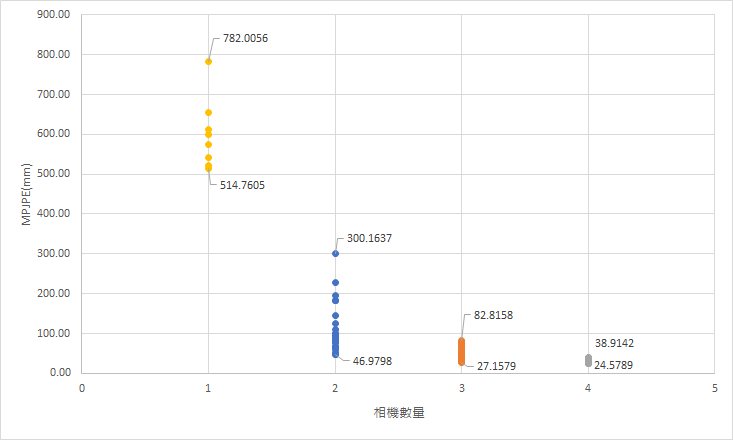
\includegraphics[width=\linewidth]{figure/ch3_fig_1to7cam.png}
   \caption[一台相機到七台相機的組合估計結果]{一台相機到七台相機的組合估計結果}
   \label{ch3_fig_1to7cam}
\end{figure}

\clearpage

% ------------------------- 4.2 ------------------------- %
\section{個人化三維人體模型建立實驗結果與討論}\label{ch4_skeleton_exp}
% 實驗設定;實驗執行;結果與討論
% 在章節~\ref{ch3_skeleton_method} 中已詳細描述了個人化三維人體模型建立的方法,
% 本節使用 TotalCapture Dataset~\cite{Trumble:BMVC:2017} 提供的影片資料及相機校正數據,
% 嘗試建立影片中受試者的個人化三維人體模型,並進行比較及討論。

\subsection{實驗設定}
% 把 total capture dataset s1 系列做完
本章節使用 TotalCapture Dataset ~\cite{Trumble:BMVC:2017} 提供的 s1\_acting1 \textasciitilde\ s1\_acting3、s1\_freestyle1 \textasciitilde\ s1\_freestyle3、s1\_rom1 \textasciitilde\ s1\_rom3 共九組影片資料及相機校正資料進行實驗,每組實驗皆取用 TotalCapture Dataset  提供的相機 1 與相機 8 之影像資料、兩台相機的校正資訊,以及 .bvh 檔案中 HIERARCHY 部分提供的 Vicon 三維人體模型資訊 (此資訊可由 Vicon 量測而得,因此以下將稱為 Vicon 三維人體模型)。首先,利用影像資料進行 OpenPose 影像辨識,再使用 Pose2Sim 進行相機校正及三角測量計算,建立出個人化三維人體模型。最後,取前 60 幀的資訊,計算個人化三維人體模型的平均四肢長度,並與 Vicon 三維人體模型的四肢長度進行比較。

\subsection{實驗結果與誤差評估}
% 個人化三維人體模型建立結果與驗證
% 分別評估四肢的誤差,然後再綜合再一起評估,總結誤差大概在多少內
分別計算出自行建立個人化三維人體模型的四肢長度及 Vicon 三維人體模型長度後,將兩者相減得到誤差,並計算平均誤差,結果如表~\ref{ch3_skeleton_compare} 所示,可以發現自行建立個人化三維人體模型之四肢長度與 Vicon 三維人體模型之四肢長度相當接近,整體平均誤差為 25.7515 (mm)。本研究推斷,此項誤差可能來自 OpenPose 自身影像辨識造成的誤差,以及相機校正及三角測量的誤差。
% \sout{因此,若要進一步提升個人化三維人體模型的精確度,可能需要改善 OpenPose 的影像辨識精度,或是改善相機校正及三角測量的精確度。}

\begin{table}[!ht]
   \caption[個人化三維人體模型建立結果與比較(mm)]{個人化三維人體模型建立結果與比較(mm)}
   \centering
   \label{ch3_skeleton_compare}
   \setlength{\tabcolsep}{3pt}
   \renewcommand\arraystretch{1.5}
   \resizebox{\textwidth}{!}{
    \begin{tabular}{c|S|S|S|S|S|S|S|S|S||S}
      & {s1\_acting1} & {s1\_acting2} & {s1\_acting3} & {s1\_freestyle1} & {s1\_freestyle2} & {s1\_freestyle3} & {s1\_rom1} & {s1\_rom2} & {s1\_rom3} & {average} \\
      \midrule[1.5pt]
      右大腿 & 15.5895 & 16.8009 & 5.8655 & 27.9576 & 24.0688 & 18.2016 & 9.7907 & 12.2067 & 1.5568 & 14.6709  \\
      右小腿 & 20.4312 & 0.7514 & 8.9552 & 11.4757 & 12.7413 & 2.5780 & 19.0733 & 20.5609 & 8.6443 & 11.6902  \\
      左大腿 & 20.1423 & 23.3496 & 14.8347 & 34.8388 & 25.4773 & 29.7342 & 18.8850 & 15.3576 & 24.7152 & 23.0372  \\
      左小腿 & 3.4795 & 7.8705 & 16.6157 & 15.0529 & 12.4442 & 15.5452 & 12.3024 & 3.2584 & 3.2571 & 9.9807  \\
      右上臂 & 37.1875 & 39.5958 & 43.2833 & 76.6637 & 59.6534 & 34.1348 & 59.4540 & 29.4289 & 32.0788 & 45.7200  \\
      右前臂 & 4.0619 & 20.9168 & 14.4801 & 59.1019 & 37.3311 & 10.6598 & 36.6949 & 4.3855 & 13.8587 & 22.3878  \\
      左上臂 & 47.6423 & 50.8824 & 51.3296 & 41.4413 & 48.9365 & 51.4196 & 36.5617 & 50.4505 & 53.2362 & 47.9889  \\
      左前臂 & 30.7583 & 24.3253 & 36.5486 & 19.8007 & 29.5842 & 34.7937 & 22.6062 & 35.9636 & 40.4441 & 30.5361  \\
      \midrule[1.5pt]
      average & 22.4116 & 23.0616 & 23.9891 & 35.7916 & 31.2796 & 24.6334 & 26.9210 & 21.4515 & 22.2239 & 25.7515  \\
   \end{tabular}}
\end{table}

\subsection{結論}
% 結論
由以上誤差評估可知,本方法的整體平均誤差約為 25.75 (mm),若僅用於建立三維人體模型、評估人體全身姿勢,不進行複雜動作的量測,使動作產生許多遮擋問題,或是延伸應用於評估手指姿勢等細微動作,則此誤差並不會造成誤判的影響,因此證明本方法確實可應用於建立三維人體模型,作為將 IMU 朝向資訊轉換為位置資訊的媒介。

\clearpage

% ------------------------- 4.3 ------------------------- %
% \section{使用影像辨識估計姿態}
% % 單獨 heatmap 的結果
% \subsection{實驗設定}
% % 實驗設定
% 本章節將自行蒐集的資料輸入進學者 Zhe Zhang 等人提出的感測器融合方法中進行人體姿態重建~\cite{Zhang_2020_CVPR}。該方法中包含兩個主要流程,一為影像辨識,二為影像辨識結果融合 IMU 資訊,本章節僅使用影像辨識進行人體姿態重建,不進行 IMU 資訊融合。使用的影像辨識方法為文獻~\cite{Xiao_2018_ECCV} 中,學者 Bin Xiao 等人提出的方法,並套用 Zhe Zhang 等人訓練的 $occlusion\_person\_8view.pth$ 模型進行影像辨識~\cite{zhang2020adafuse},取得記錄關節點於影像中位置的初步熱圖後,使用三角測量方法計算關節點的三維位置,進而重建人體姿態。

% % \subsection{實驗執行}
% % % 實驗執行

% \subsection{實驗結果與誤差評估}
% \subsubsection*{T pose實驗結果}
% % 用pose_41、273
% 使用影像辨識融合 IMU 資訊的 T pose 重建結果如圖~\ref{ch4_fig_Tpose_noimu} 所示,(a)、(b) 為同一時刻點的 cam01 影像及 cam02 影像,(c) 為人體重建結果;(c)、(d) 為同一時刻點的 cam01 影像及 cam02 影像,(e) 為人體重建結果。可以發現,在第二個時刻的 T pose 人體重建結果與真實人體姿態有些出入。
% \begin{figure}[!ht]
%    \centering
%    \begin{minipage}{.3\textwidth}
%      \centering
%      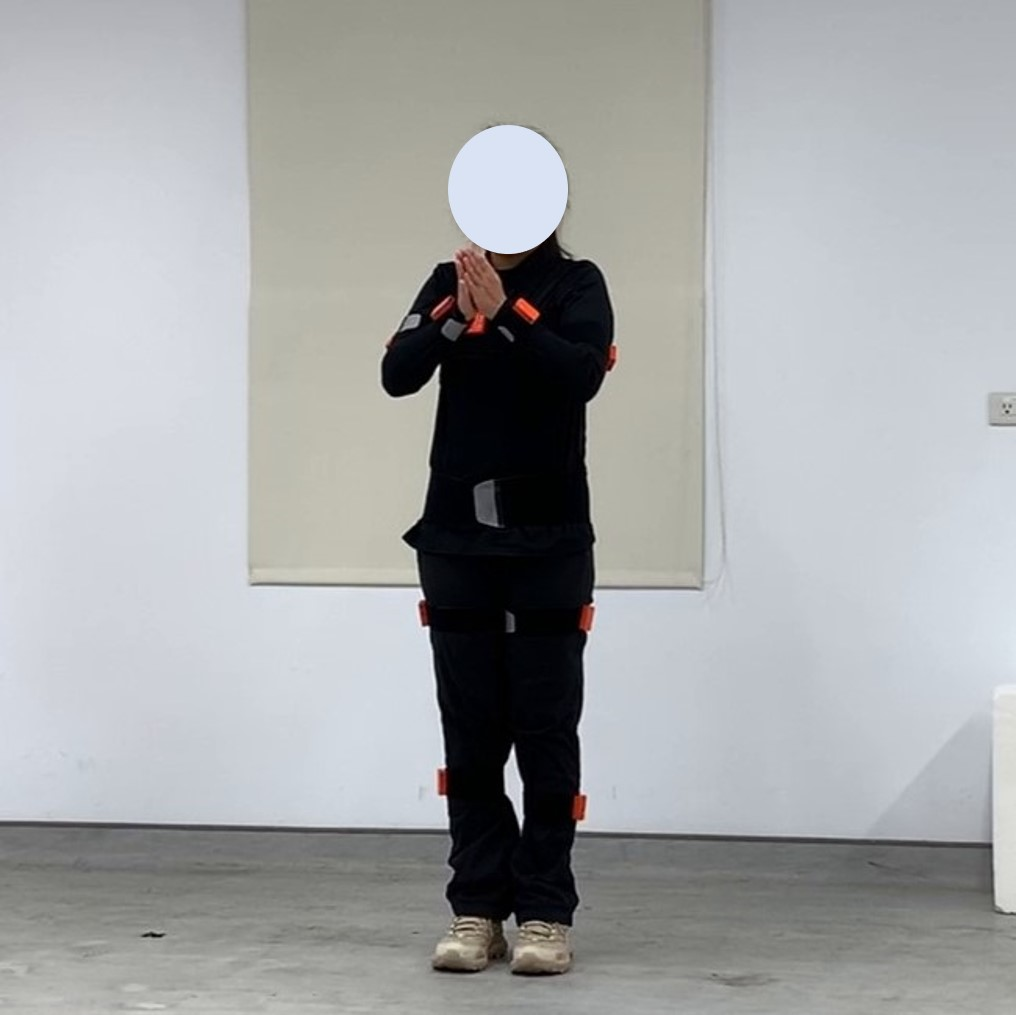
\includegraphics[width=\linewidth]{figure/ch4_fig_tpose_cam01_no1.jpg}
%      \caption*{(a) cam01 真實影像}
%    \end{minipage}%
%    \begin{minipage}{.3\textwidth}
%       \centering
%       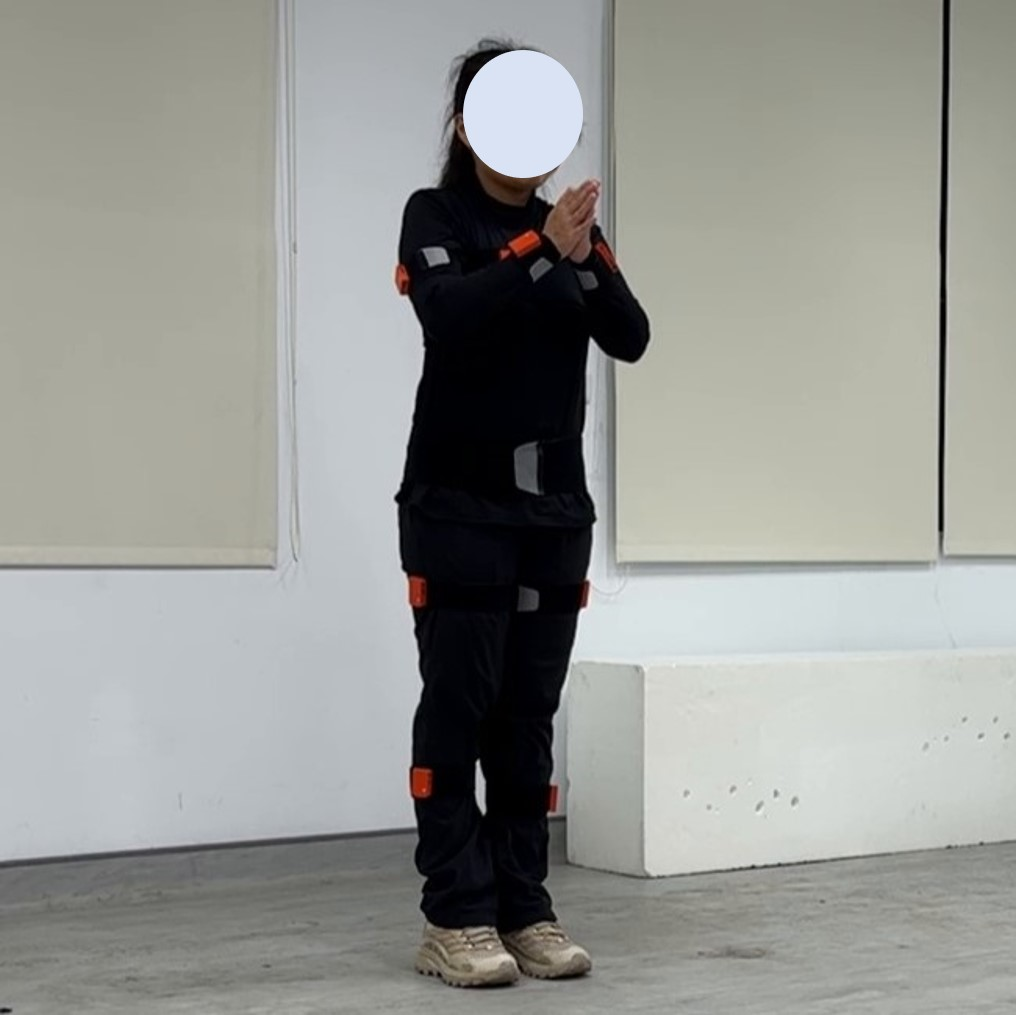
\includegraphics[width=\linewidth]{figure/ch4_fig_tpose_cam02_no1.jpg}
%       \caption*{(b) cam02 真實影像}
%    \end{minipage}%
%    \begin{minipage}{.3\textwidth}
%       \centering
%       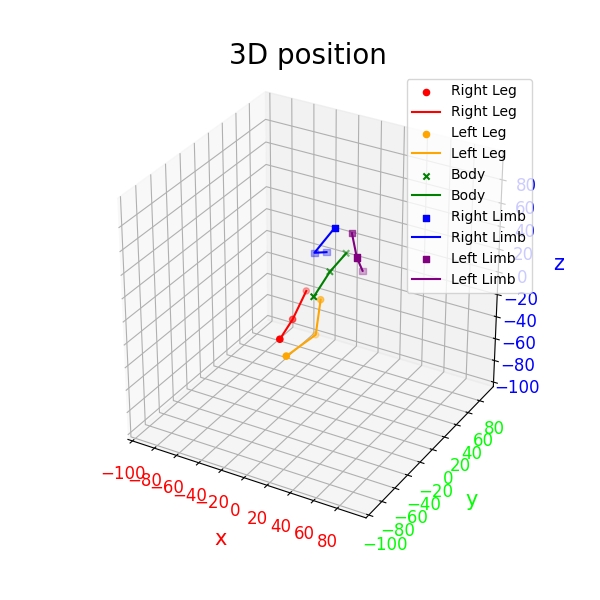
\includegraphics[width=\linewidth]{figure/ch4_fig_tpose_result_no1.png}
%       \caption*{(c) 重建結果}
%    \end{minipage}
%    \begin{minipage}{.3\textwidth}
%      \centering
%      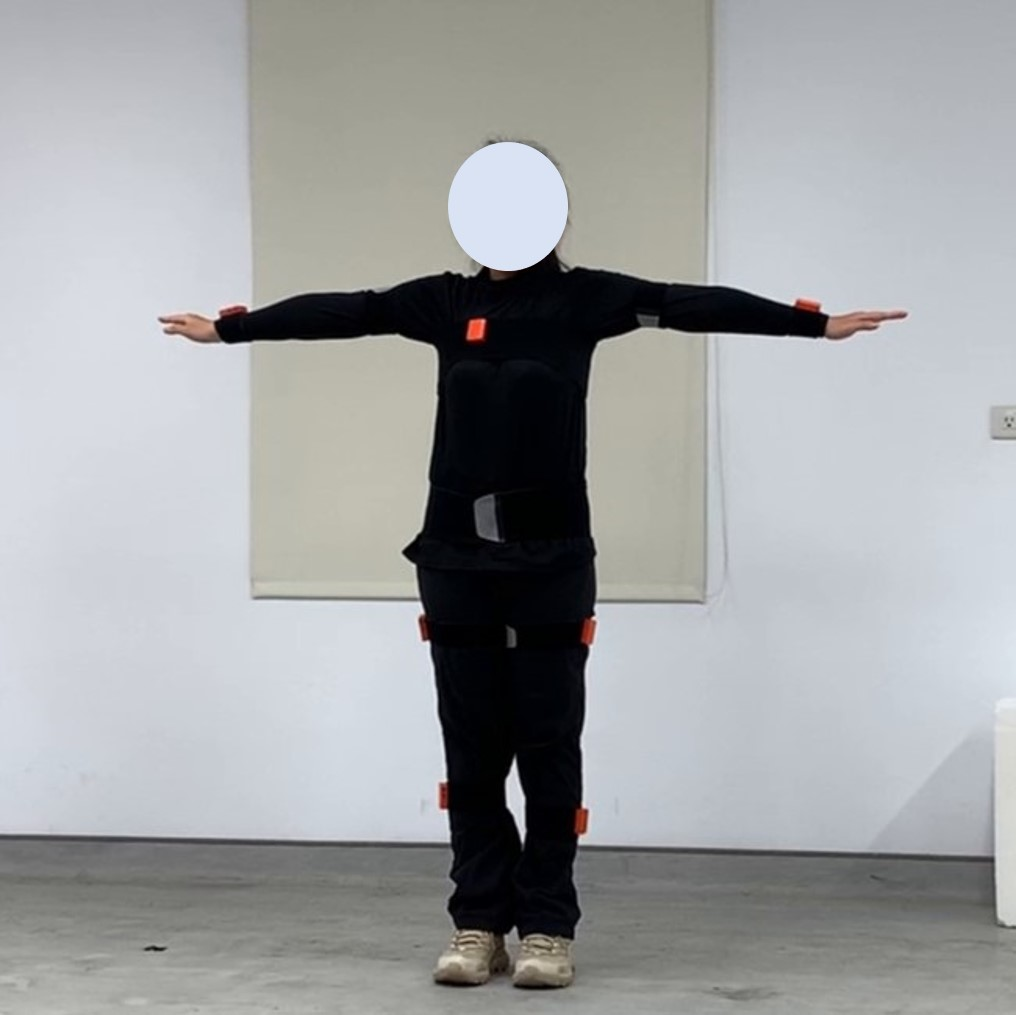
\includegraphics[width=\linewidth]{figure/ch4_fig_tpose_cam01_no2.jpg}
%      \caption*{(d) cam01 真實影像}
%    \end{minipage}%
%    \begin{minipage}{.3\textwidth}
%       \centering
%       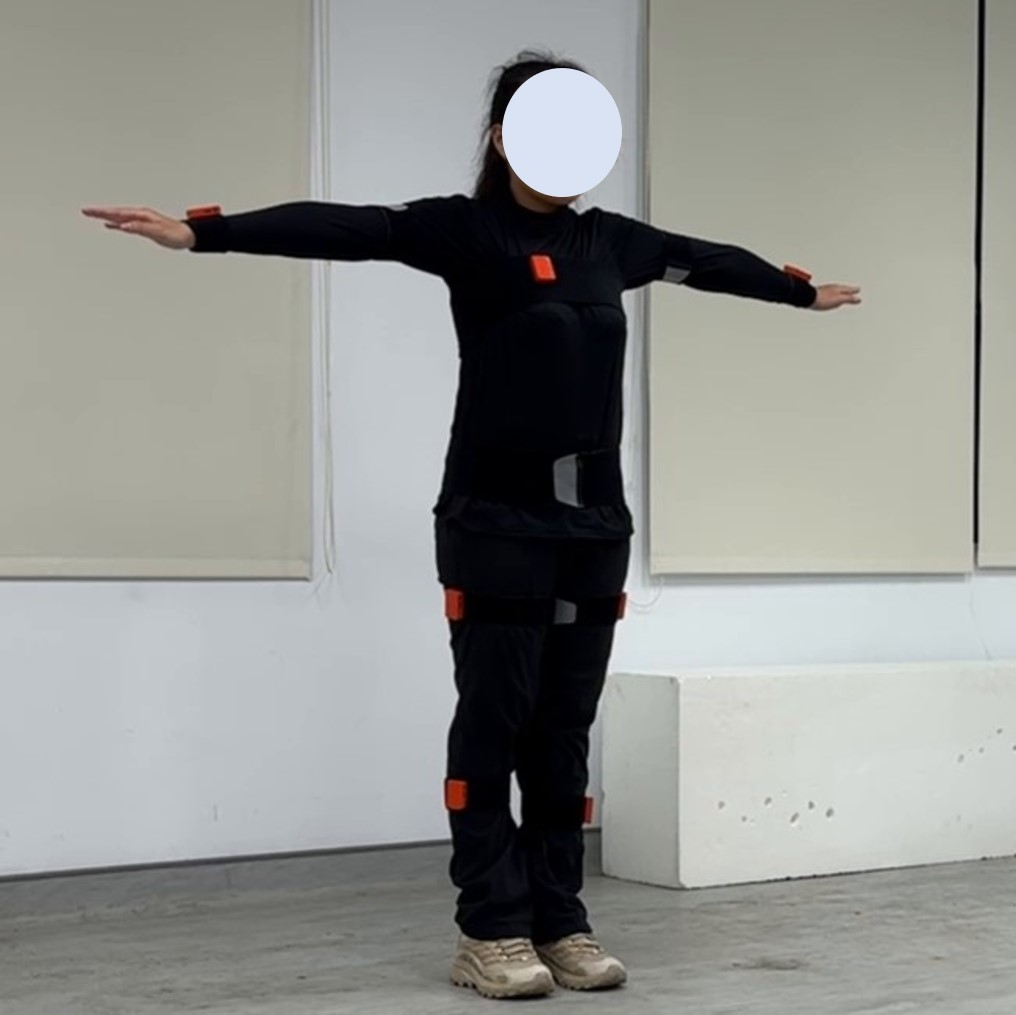
\includegraphics[width=\linewidth]{figure/ch4_fig_tpose_cam02_no2.jpg}
%       \caption*{(e) cam02 真實影像}
%     \end{minipage}%
%     \begin{minipage}{.3\textwidth}
%       \centering
%       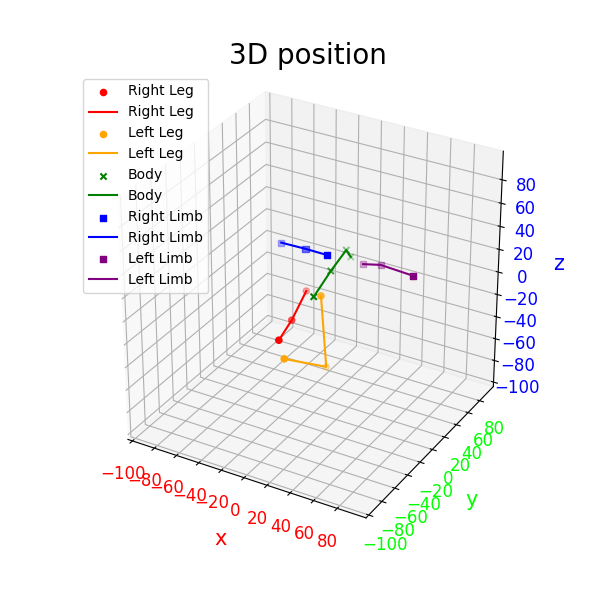
\includegraphics[width=\linewidth]{figure/ch4_fig_tpose_result_no2.png}
%       \caption*{(f) 重建結果}
%     \end{minipage}
%    \caption[僅使用影像辨識進行 T pose 重建結果]{僅使用影像辨識進行 T pose 重建結果}
%    \label{ch4_fig_Tpose_noimu}
% \end{figure}

% \subsubsection*{T pose 誤差評估}
% T pose 實驗總計有 318 幀,每一幀皆估計出人體姿態,每 20 幀進行一次採樣,共計 16 個樣本點進行評估及驗證,
% % 結果如表~\ref{ch4_Tpose_result_noimu} 所示,
% 可以發現,T pose 實驗中,肢段的平均估計成功率約 12.5\%,平均有效誤差約在 95.0632 (mm)。

% % \begin{table}[!ht]
% %    \caption[影像辨識 T pose 實驗結果與誤差評估]{影像辨識 T pose 實驗結果與誤差評估}
% %    \centering
% %    \label{ch4_Tpose_result_noimu}
% %    \setlength{\tabcolsep}{3pt}
% %    \renewcommand\arraystretch{1.5}
% %    \resizebox{\textwidth}{!}{
% %    \begin{tabular}{c|c|c|c|c|c|c|c|c|c}
% %       & {右大腿} & {右小腿} & {左大腿} & {左小腿} & {右上臂} & {右前臂} & {左上臂} & {左前臂} & {平均} \\
% %       \midrule[1.5pt]
% %       成功幀數 & 304 & 187 & 16 & 12 & 61 & 92 & 183 & 273 & \\
% %       成功率 & 95.59 & 58.81 & 5.03 & 3.77 & 57.55 & 85.85 & 19.18 & 28.93 & 44.34 \\
% %       \midrule
% %       平均估計長度 & \num{301.1909} & \num{274.8160} & \num{351.1900} & \num{442.4955} & \num{267.7453} & \num{227.7233} & \num{237.5203} & \num{258.1625} & \\
% %       估計誤差 & \num{73.0909} & \num{85.1839} & \num{13.8100} & \num{77.4955} & \num{39.2547} & \num{12.7233} & \num{57.4797} & \num{47.1625} & \num{50.7751} \\
% %    \end{tabular}}
% % \end{table}

% \subsubsection*{蹲站實驗結果}
% % 用pose_59、172
% 使用影像辨識融合 IMU 資訊的蹲站重建結果如圖~\ref{ch4_fig_bar_noimu} 所示,(a)、(b) 為同一時刻點的 cam01 影像及 cam02 影像,(c) 為人體重建結果;(c)、(d) 為同一時刻點的 cam01 影像及 cam02 影像,(e) 為人體重建結果。可以發現,兩個時刻的蹲站的人體重建結果相當接近真實人體姿態。
% \begin{figure}[!ht]
%    \centering
%    \begin{minipage}{.3\textwidth}
%      \centering
%      \includegraphics[width=\linewidth]{figure/ch4_fig_bar_cam01_no1.jpg}
%      \caption*{(a) cam01 真實影像}
%    \end{minipage}%
%    \begin{minipage}{.3\textwidth}
%       \centering
%       \includegraphics[width=\linewidth]{figure/ch4_fig_bar_cam02_no1.jpg}
%       \caption*{(b) cam02 真實影像}
%    \end{minipage}%
%    \begin{minipage}{.3\textwidth}
%       \centering
%       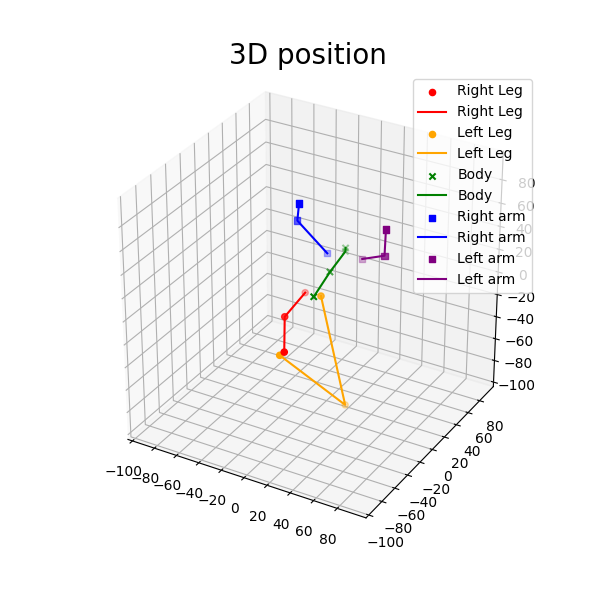
\includegraphics[width=\linewidth]{figure/ch4_fig_bar_result_no1.png}
%       \caption*{(c) 重建結果}
%    \end{minipage}
%    \begin{minipage}{.3\textwidth}
%      \centering
%      \includegraphics[width=\linewidth]{figure/ch4_fig_bar_cam01_no2.jpg}
%      \caption*{(d) cam01 真實影像}
%    \end{minipage}%
%    \begin{minipage}{.3\textwidth}
%       \centering
%       \includegraphics[width=\linewidth]{figure/ch4_fig_bar_cam02_no2.jpg}
%       \caption*{(e) cam02 真實影像}
%     \end{minipage}%
%     \begin{minipage}{.3\textwidth}
%       \centering
%       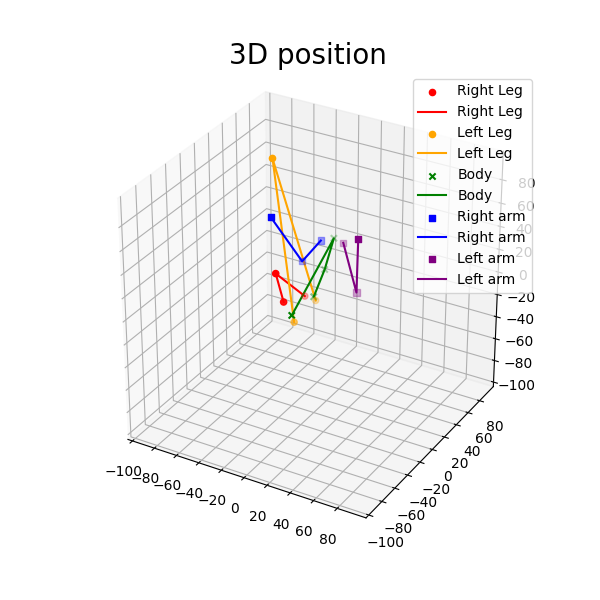
\includegraphics[width=\linewidth]{figure/ch4_fig_bar_result_no2.png}
%       \caption*{(f) 重建結果}
%     \end{minipage}
%    \caption[僅使用影像辨識進行蹲站重建結果]{僅使用影像辨識進行蹲站重建結果}
%    \label{ch4_fig_bar_noimu}
% \end{figure}

% \subsubsection*{蹲站誤差評估}
% 蹲站實驗總計有 1245 幀,每一幀皆估計出人體姿態,每 20 幀進行一次採樣,共計 63 個樣本點進行評估及驗證,可以發現,蹲站實驗中,肢段的平均估計成功率約 11.11\%,平均有效誤差約在 94.5808 (mm)。

% \subsubsection*{開合跳實驗結果}
% \subsubsection*{開合跳誤差評估}
% \subsubsection*{折返跑實驗結果}
% \subsubsection*{折返跑誤差評估}
% \subsubsection*{熱身運動實驗結果}
% \subsubsection*{熱身運動誤差評估}
% \subsubsection*{組合動作實驗結果}
% \subsubsection*{組合動作誤差評估}

% \subsection{結論}
% % 結論
% 123123

% % ------------------------- 4.3 ------------------------- %
% \section{單獨做 IMU 的姿勢估計}
% 單獨 IMU 的結果
% \subsection{實驗設定}
% % 實驗設定
% 123123
% \subsection{實驗執行}
% % 實驗執行
% 123123
% \subsection{誤差評估}
% % 誤差評估
% 123123
% \subsection{結論}
% % 結論
% 123123

% ------------------------- 4.3 ------------------------- %
\section{使用影像辨識融合 IMU 估計姿態}
% sensor fusion 在室內的結果
\subsection{實驗設定}
% 實驗設定
本章節將自行蒐集的資料輸入進學者 Zhe Zhang 等人提出的感測器融合方法中進行人體姿態重建~\cite{Zhang_2020_CVPR}。該方法中包含兩個主要流程,一為影像辨識,二為影像辨識結果融合 IMU 資訊,本章節使用的影像辨識方法為文獻~\cite{Xiao_2018_ECCV} 中,學者 Bin Xiao 等人提出的方法,並套用 Zhe Zhang 等人訓練的 $occlusion\_person\_8view.pth$ 模型進行影像辨識~\cite{zhang2020adafuse},取得記錄關節點於影像中位置的初步熱圖,接著選擇是否融合 IMU 資訊,最後使用三角測量方法計算關節點的三維位置,進而重建人體姿態。

% \subsection{實驗執行}
% % 實驗執行

\subsection{實驗結果與誤差評估}
\subsubsection*{T pose 實驗結果}
% 用pose_59、172
T pose 重建結果如圖~\ref{ch4_fig_Tpose} 所示,(a)、(b) 為同一時刻點的 cam01 影像及 cam02 影像,(c) 為使用影像辨識融合 IMU 資訊的人體重建結果,(d) 為僅使用影像辨識的人體重建結果。
% ;(e)、(f) 為同一時刻點的 cam01 影像及 cam02 影像,(g) 為使用影像辨識融合 IMU 資訊的人體重建結果,(h) 為僅使用影像辨識的人體重建結果。

\begin{figure}[!ht]
   \centering
   % \begin{minipage}{.25\textwidth}
   %   \centering
   %   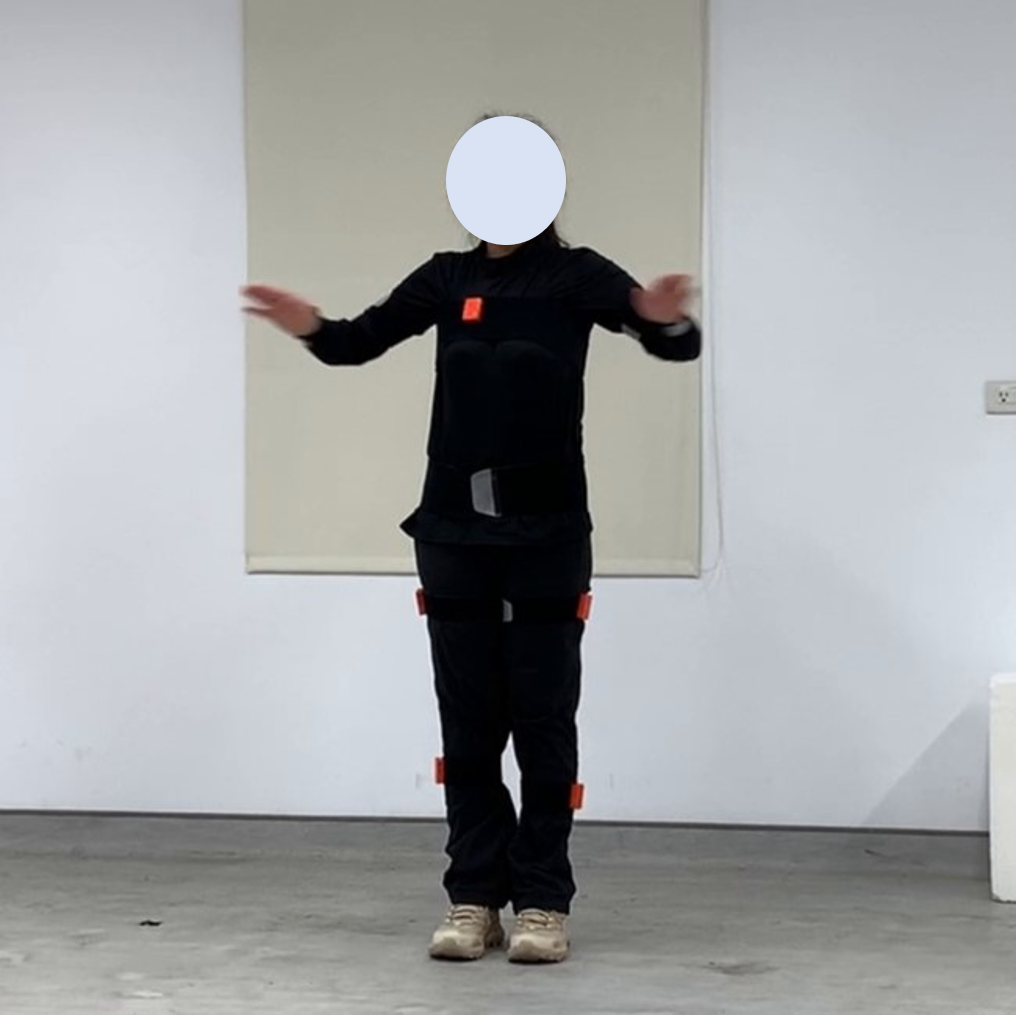
\includegraphics[width=\linewidth]{figure/ch4_fig_tpose_cam01_with1.jpg}
   %   \caption*{(a) cam01 真實影像}
   % \end{minipage}%
   % \begin{minipage}{.25\textwidth}
   %    \centering  
   %    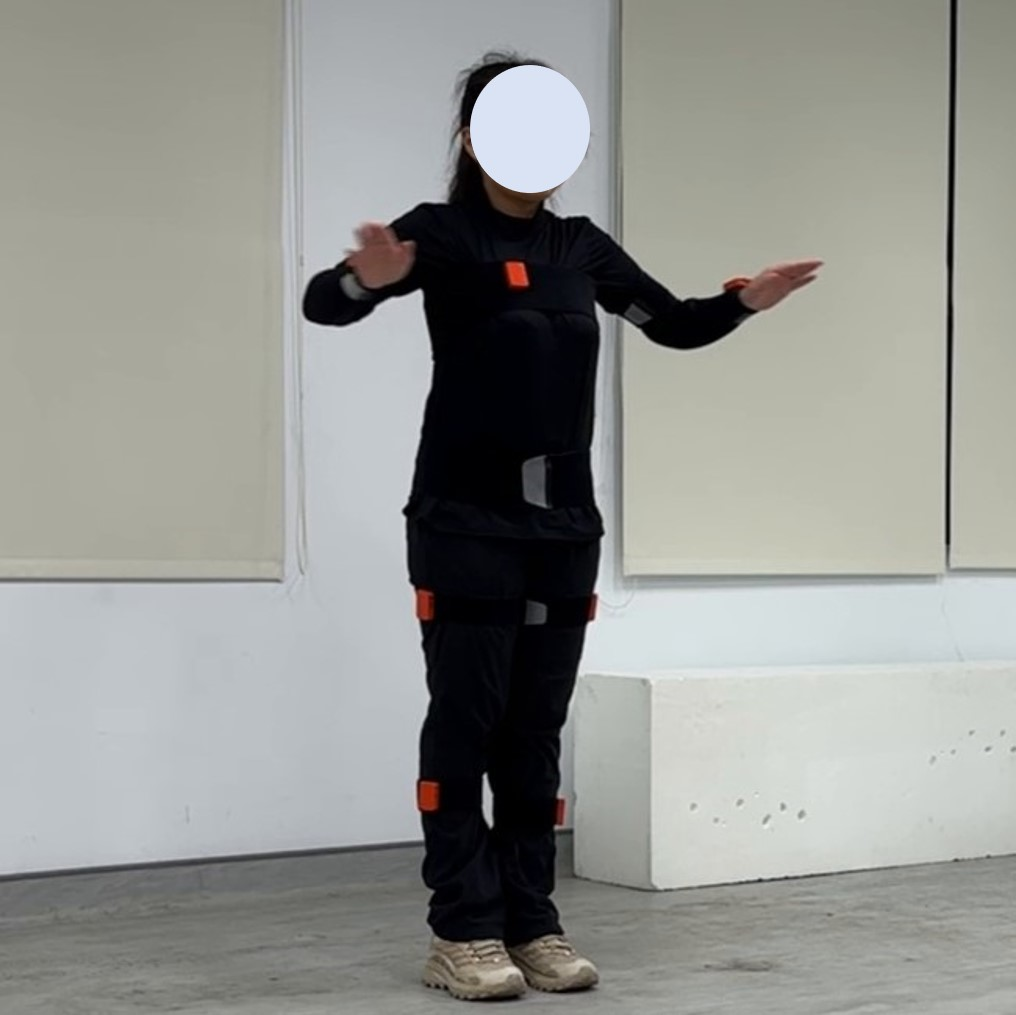
\includegraphics[width=\linewidth]{figure/ch4_fig_tpose_cam02_with1.jpg}
   %    \caption*{(b) cam02 真實影像}
   % \end{minipage}%
   % \begin{minipage}{.25\textwidth}
   %    \centering
   %    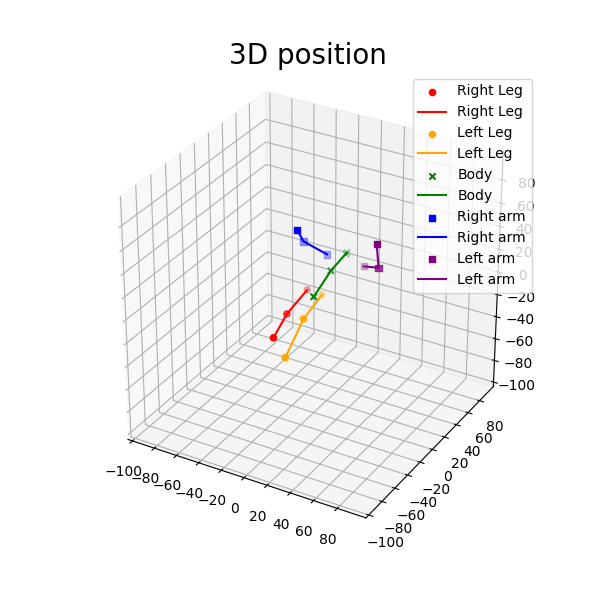
\includegraphics[width=\linewidth]{figure/ch4_fig_tpose_result_with1.png}
   %    \caption*{(c) 影像辨識融合 IMU 重建結果}
   % \end{minipage}%
   % \begin{minipage}{.25\textwidth}
   %    \centering
   %    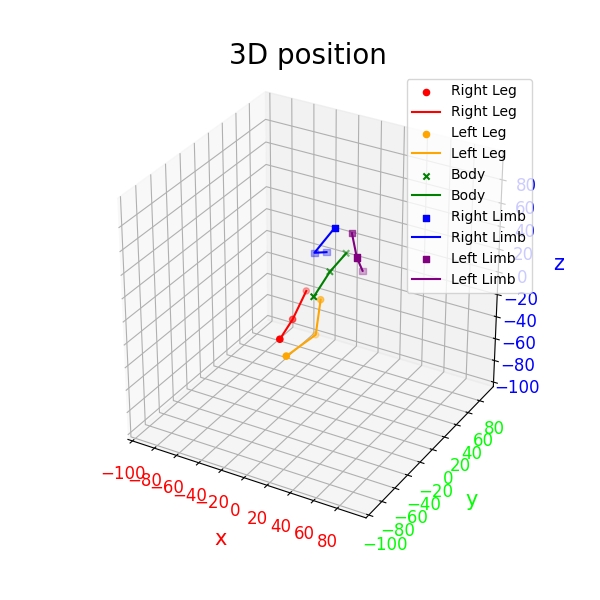
\includegraphics[width=\linewidth]{figure/ch4_fig_tpose_result_no1.png}
   %    \caption*{(d) 影像辨識重建結果}
   % \end{minipage}
   \begin{minipage}{.5\textwidth}
     \centering
     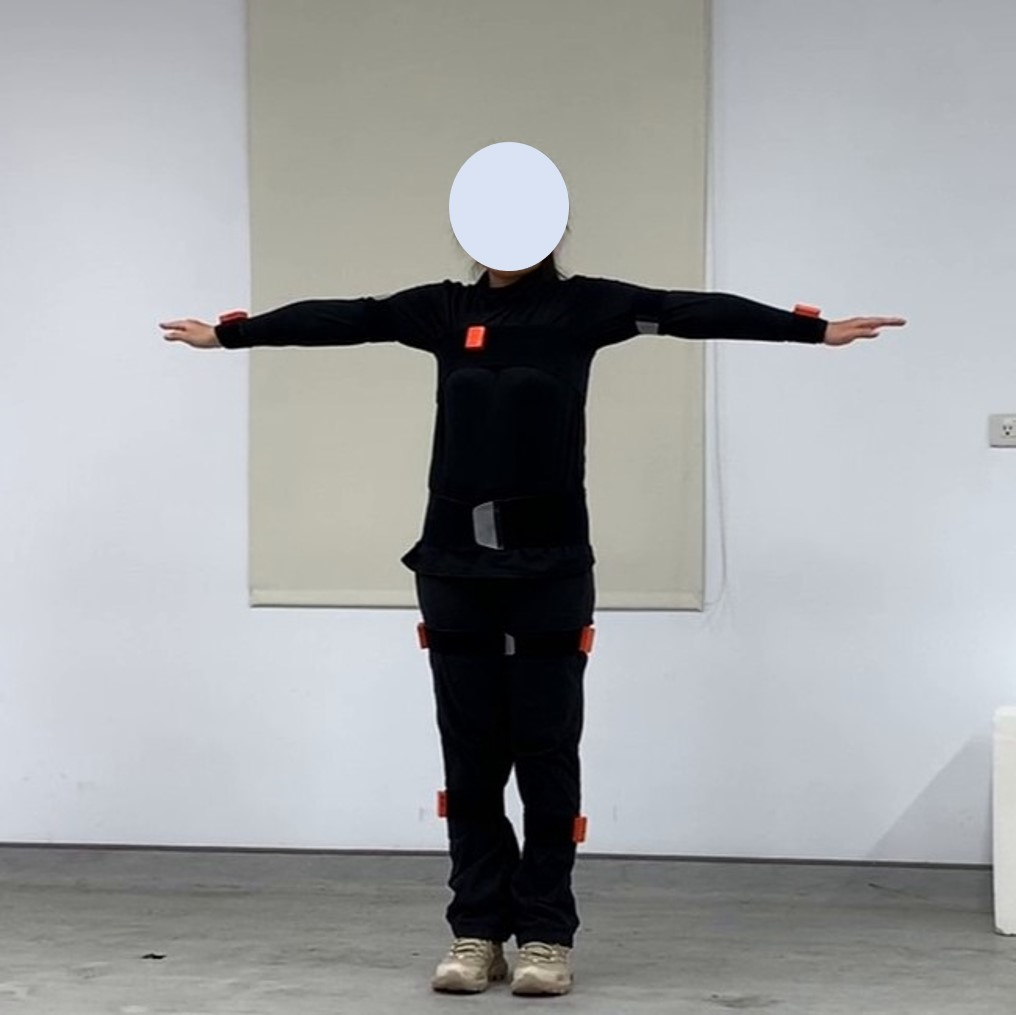
\includegraphics[width=.95\linewidth]{figure/ch4_fig_tpose_cam01_with2.jpg}
     \caption*{(a) cam01 真實影像}
   \end{minipage}%
   \begin{minipage}{.5\textwidth}
      \centering
      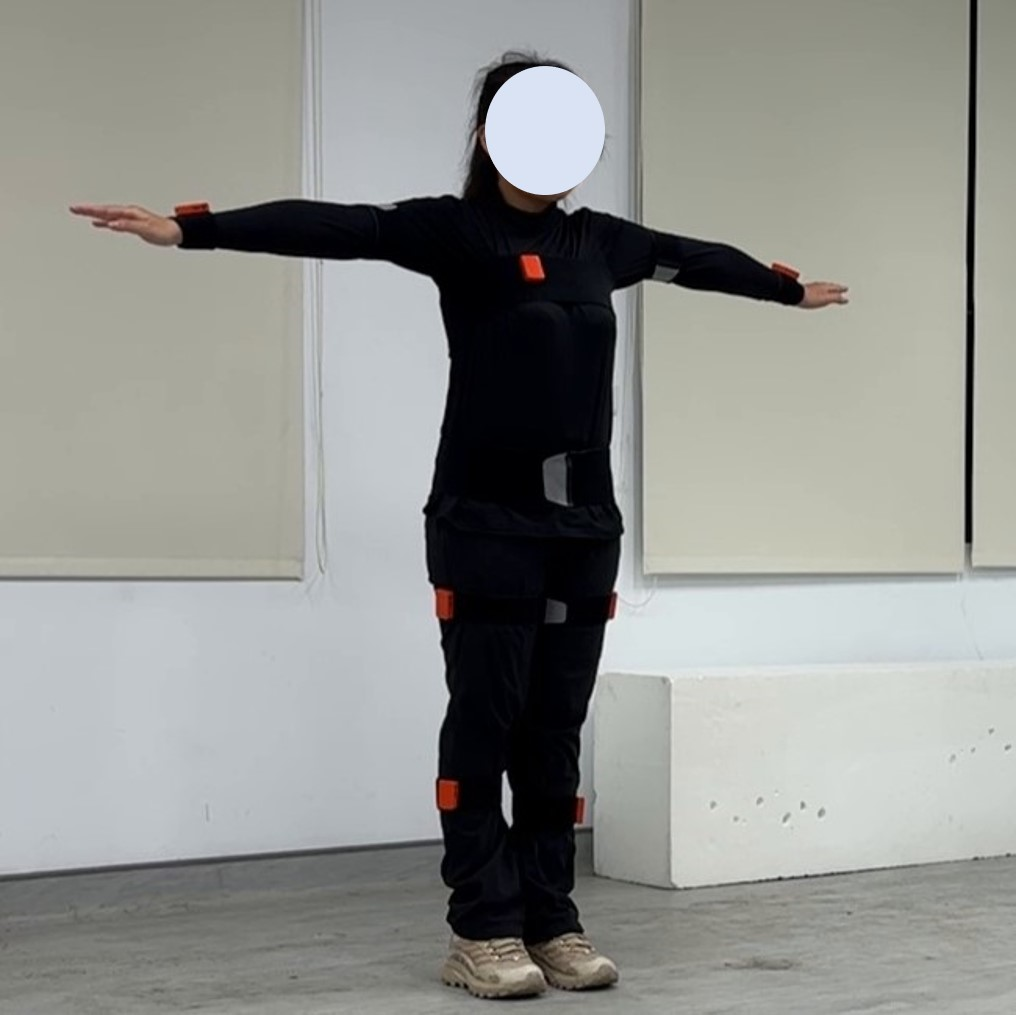
\includegraphics[width=.95\linewidth]{figure/ch4_fig_tpose_cam02_with2.jpg}
      \caption*{(b) cam02 真實影像}
   \end{minipage}
   \begin{minipage}{.5\textwidth}
      \centering
      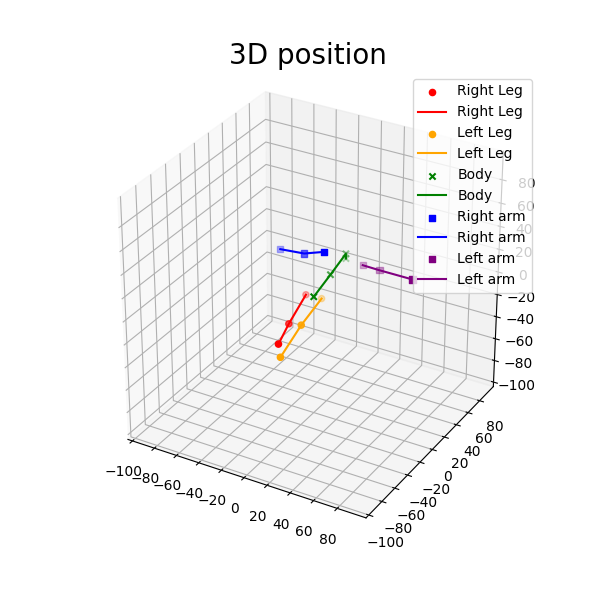
\includegraphics[width=.95\linewidth]{figure/ch4_fig_tpose_result_with2.png}
      \caption*{(c) 影像辨識融合 IMU 重建結果}
   \end{minipage}%
   \begin{minipage}{.5\textwidth}
      \centering
      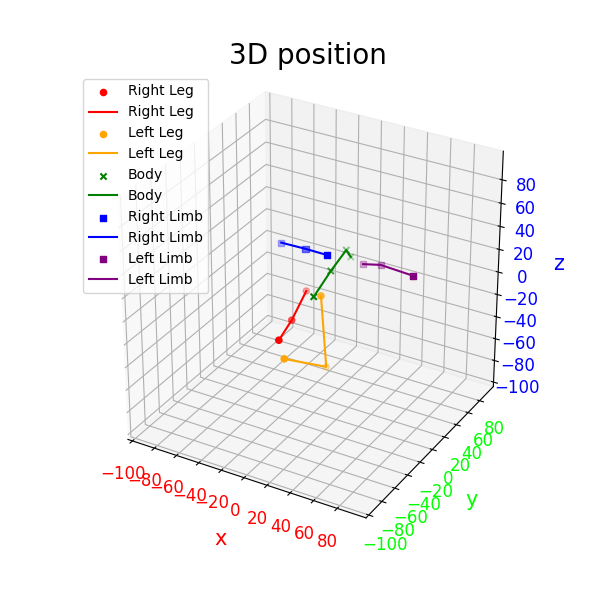
\includegraphics[width=.95\linewidth]{figure/ch4_fig_tpose_result_no2.png}
      \caption*{(d) 影像辨識重建結果}
   \end{minipage}
   \caption[T pose 重建結果]{T pose 重建結果}
   \label{ch4_fig_Tpose}
\end{figure}

\subsubsection*{T pose 誤差評估}
T pose 實驗總計有 318 幀,每一幀皆估計出人體姿態,每 20 幀進行一次採樣,共計 16 個樣本點進行評估及驗證,
% 結果如表~\ref{ch4_Tpose_result_withimu} 所示,
可以發現,T pose 實驗中,影像辨識融合 IMU 資訊的肢段的平均估計成功率約 62.5\%,平均有效誤差約在 82.7502 (mm)。僅使用影像辨識的肢段的平均估計成功率約 12.5\%,平均有效誤差約在 95.0632 (mm)。比較圖~\ref{ch4_fig_Tpose} (c)、(d) 可以發現,僅使用影像辨識建立出來的結果關節點位置會亂飄,影像辨識融合 IMU 朝向資訊的人體重建結果較為接近真實人體姿態。

% \begin{table}[!ht]
%    \caption[影像辨識與 IMU 融合 T pose 實驗結果與誤差評估]{影像辨識與 IMU 融合 T pose 實驗結果與誤差評估}
%    \centering
%    \label{ch4_Tpose_result_withimu}
%    \setlength{\tabcolsep}{3pt}
%    \renewcommand\arraystretch{1.5}
%    \resizebox{\textwidth}{!}{
%    \begin{tabular}{c|c|c|c|c|c|c|c|c|c}
%       & {右大腿} & {右小腿} & {左大腿} & {左小腿} & {右上臂} & {右前臂} & {左上臂} & {左前臂} & {平均} \\
%       \midrule[1.5pt]
%       成功幀數 & 317 & 91 & 257 & 245 & 176 & 245 & 41 & 137 & \\
%       成功率 & 99.7 & 28.61 & 80.82 & 77.04 & 55.35 & 77.04 & 12.89 & 43.08 & 59.31 \\
%       \midrule
%       平均估計長度 & \num{322.2769} & \num{277.9209} & \num{328.7976} & \num{295.7648} & \num{273.7784} & \num{227.1334} & \num{238.0457} & \num{277.4777} & \\
%       估計誤差 & \num{52.2303} & \num{82.0791} & \num{36.2124} & \num{69.2352} & \num{33.2216} & \num{12.1334} & \num{56.9543} & \num{66.4777} & \num{51.0680} \\
%    \end{tabular}}
% \end{table}

\clearpage

\subsubsection*{蹲站實驗結果}
% 用pose_225、488
蹲站重建中,站立的實驗結果如圖~\ref{ch4_fig_bar_stand} 所示,(a)、(b) 為同一時刻點的 cam01 影像及 cam02 影像,(c) 為使用影像辨識融合 IMU 資訊的人體重建結果,(d) 為僅使用影像辨識的人體重建結果。

\begin{figure}[!ht]
   \centering
   \begin{minipage}{.5\textwidth}
      \centering
      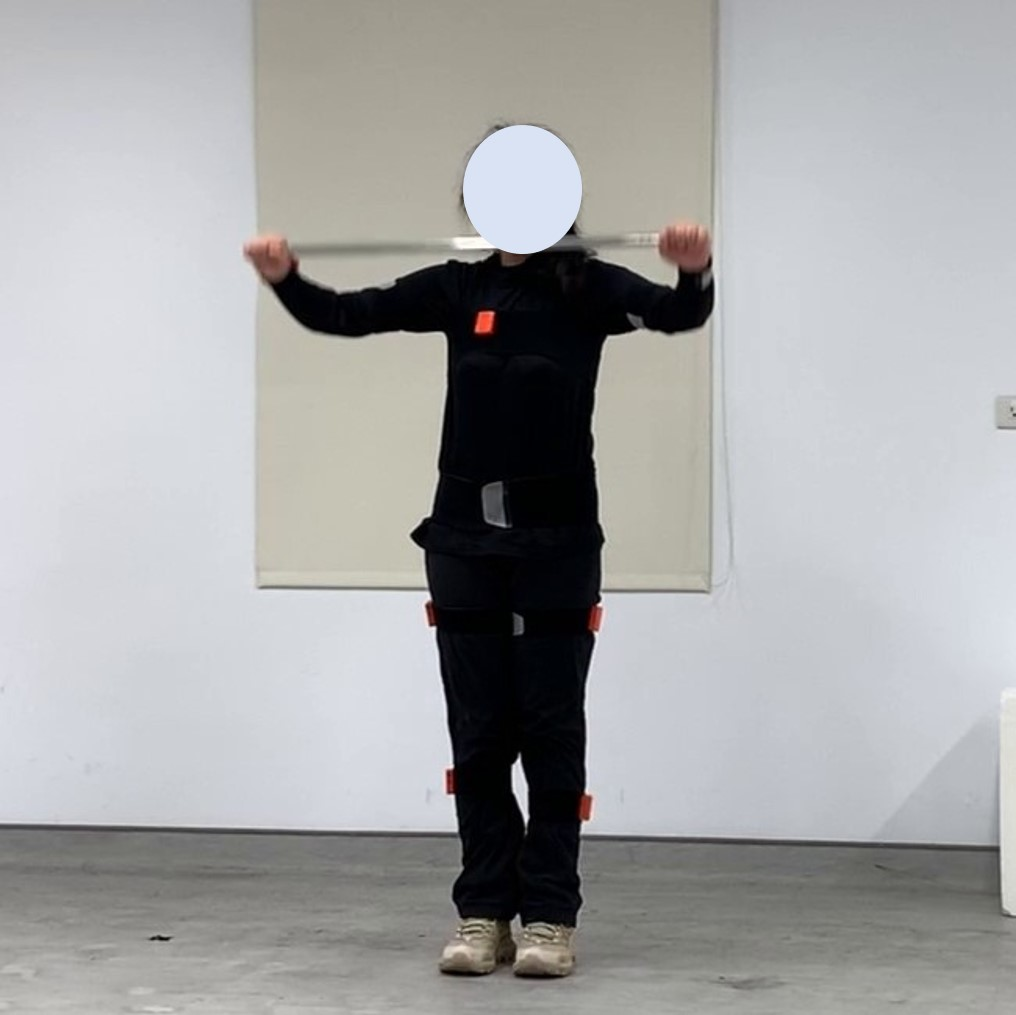
\includegraphics[width=.95\linewidth]{figure/ch4_fig_bar_cam01_with1.jpg}
      \caption*{(a) cam01 真實影像}
    \end{minipage}%
    \begin{minipage}{.5\textwidth}
       \centering
       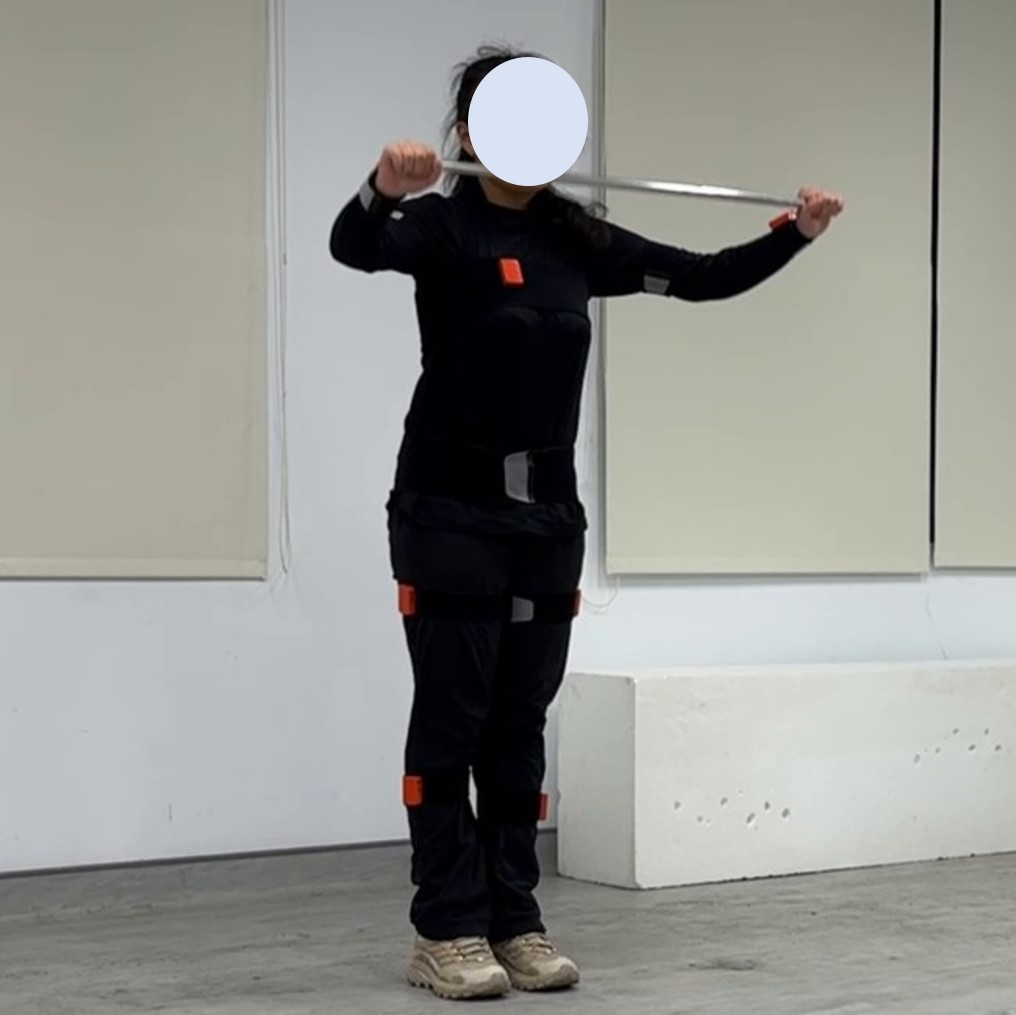
\includegraphics[width=.95\linewidth]{figure/ch4_fig_bar_cam02_with1.jpg}
       \caption*{(b) cam02 真實影像}
    \end{minipage}
    \begin{minipage}{.5\textwidth}
       \centering
       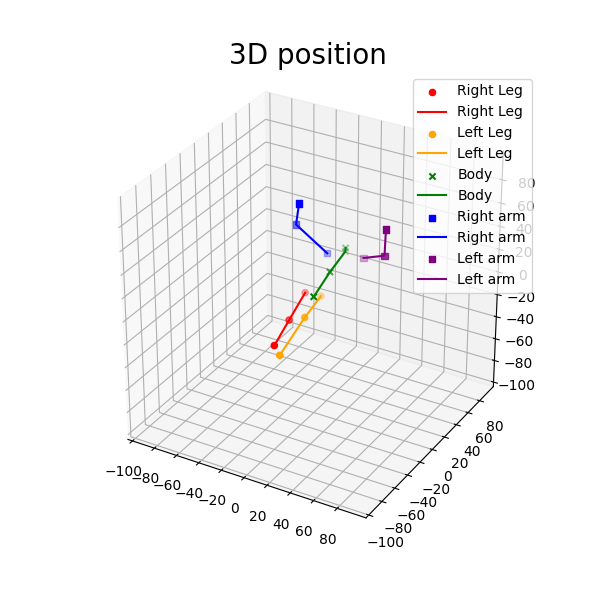
\includegraphics[width=.95\linewidth]{figure/ch4_fig_bar_result_with1.png}
       \caption*{(c) 影像辨識融合 IMU 重建結果}
    \end{minipage}%
    \begin{minipage}{.5\textwidth}
       \centering
       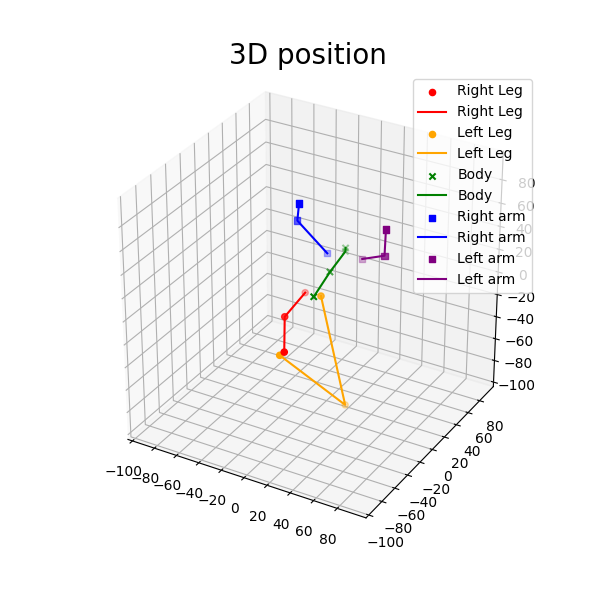
\includegraphics[width=.95\linewidth]{figure/ch4_fig_bar_result_no1.png}
       \caption*{(d) 影像辨識重建結果}
    \end{minipage}
   \caption[蹲站中站立的重建結果]{蹲站中站立的重建結果}
   \label{ch4_fig_bar_stand}
\end{figure}

\clearpage

蹲下的實驗結果如圖~\ref{ch4_fig_bar_squat} 所示,(a)、(b) 為同一時刻點的 cam01 影像及 cam02 影像,(c) 為使用影像辨識融合 IMU 資訊的人體重建結果,(d) 為僅使用影像辨識的人體重建結果。

\begin{figure}[!ht]
   \centering
   \begin{minipage}{.5\textwidth}
      \centering
      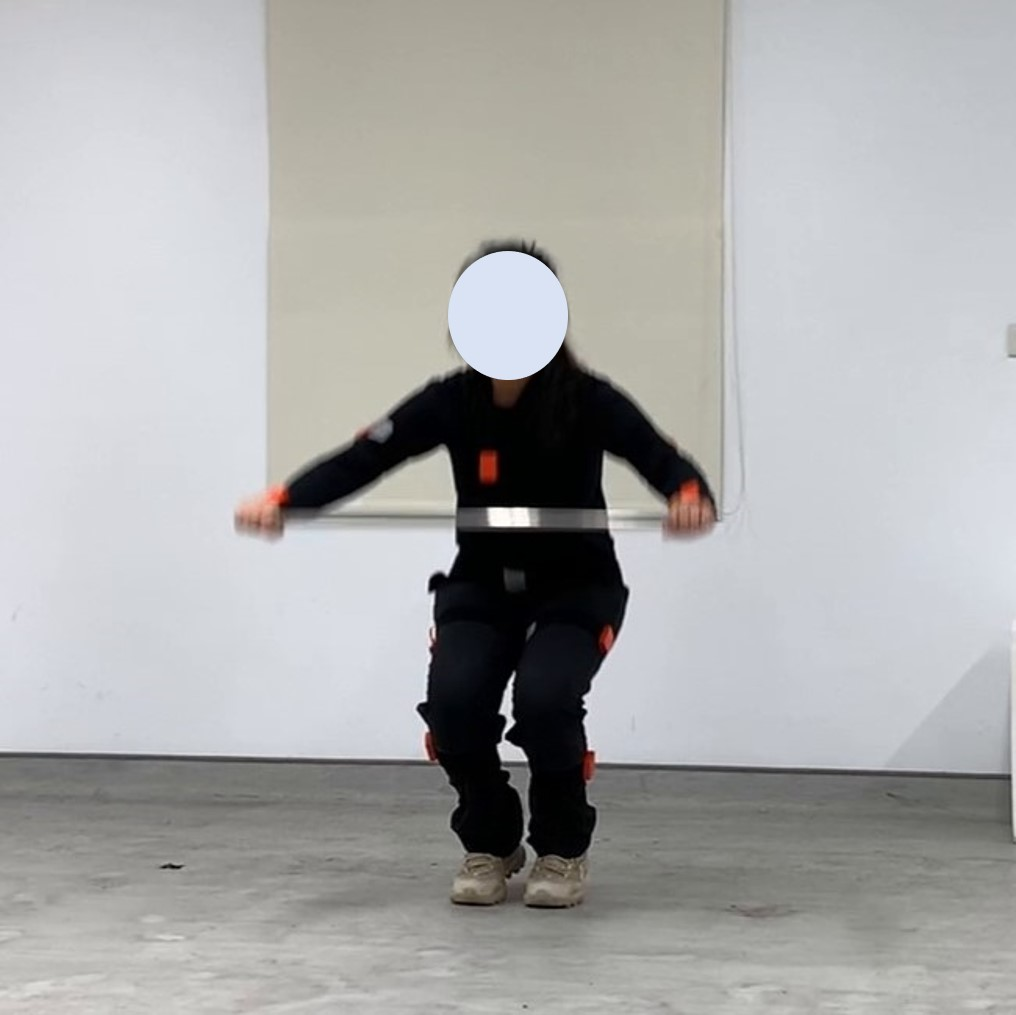
\includegraphics[width=.95\linewidth]{figure/ch4_fig_bar_cam01_with2.jpg}
      \caption*{(a) cam01 真實影像}
    \end{minipage}%
    \begin{minipage}{.5\textwidth}
       \centering
       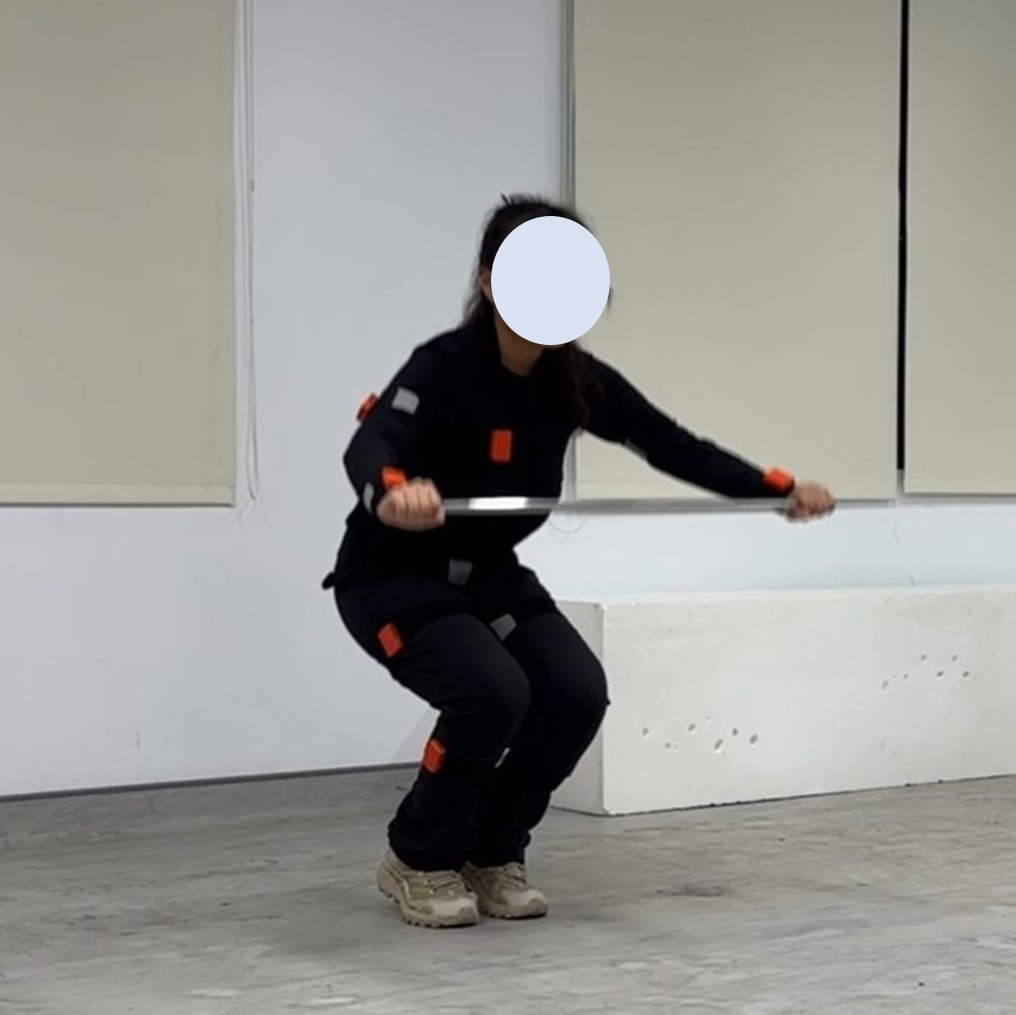
\includegraphics[width=.95\linewidth]{figure/ch4_fig_bar_cam02_with2.jpg}
       \caption*{(b) cam02 真實影像}
    \end{minipage}
    \begin{minipage}{.5\textwidth}
       \centering
       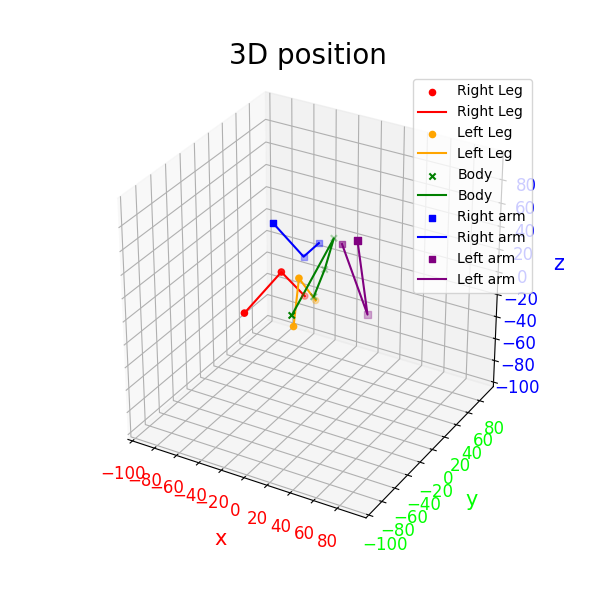
\includegraphics[width=.95\linewidth]{figure/ch4_fig_bar_result_with2.png}
       \caption*{(c) 影像辨識融合 IMU 重建結果}
    \end{minipage}%
    \begin{minipage}{.5\textwidth}
       \centering
       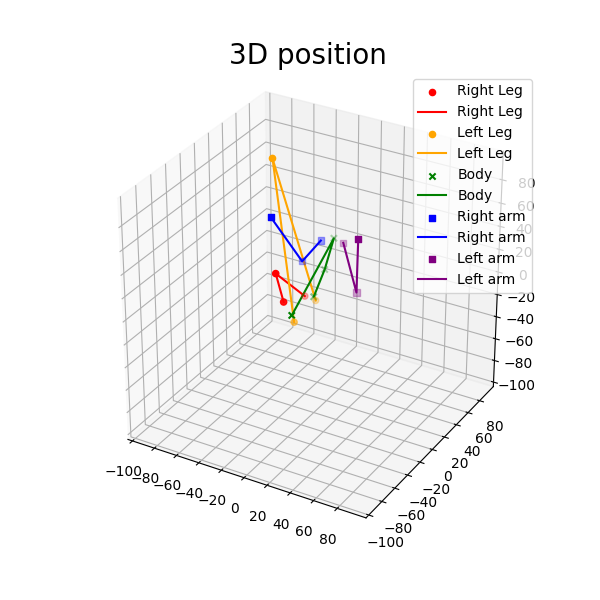
\includegraphics[width=.95\linewidth]{figure/ch4_fig_bar_result_no2.png}
       \caption*{(d) 影像辨識重建結果}
    \end{minipage}
   \caption[蹲站中蹲下的重建結果]{蹲站中蹲下的重建結果}
   \label{ch4_fig_bar_squat}
\end{figure}

\subsubsection*{蹲站誤差評估}
蹲站實驗總計有 1245 幀,每一幀皆估計出人體姿態,每 20 幀進行一次採樣,共計 63 個樣本點進行評估及驗證,可以發現,蹲站實驗中,影像辨識融合 IMU 資訊的肢段的平均估計成功率約 38.1\%,平均有效誤差約在 76.8410 (mm),僅使用影像辨識的肢段的平均估計成功率約 11.11\%,平均有效誤差約在 94.5808 (mm)。從圖~\ref{ch4_fig_bar_stand}、圖~\ref{ch4_fig_bar_squat} (c)、(d) 可以發現,僅使用影像辨識建立的關節點容易亂飄,影像辨識融合 IMU 朝向資訊的人體重建結果,由於加上朝向的限制,所以較為接近真實人體姿態。

\clearpage

\subsubsection*{開合跳實驗結果}
% pose_111、385,候選156.452.449
開合跳實驗重建中,跳起時的實驗結果如圖~\ref{ch4_fig_jump_jump} 所示,(a)、(b) 為同一時刻點的 cam01 影像及 cam02 影像,(c) 為使用影像辨識融合 IMU 資訊的人體重建結果,(d) 為僅使用影像辨識的人體重建結果。

\begin{figure}[!ht]
   \centering
   \begin{minipage}{.5\textwidth}
      \centering
      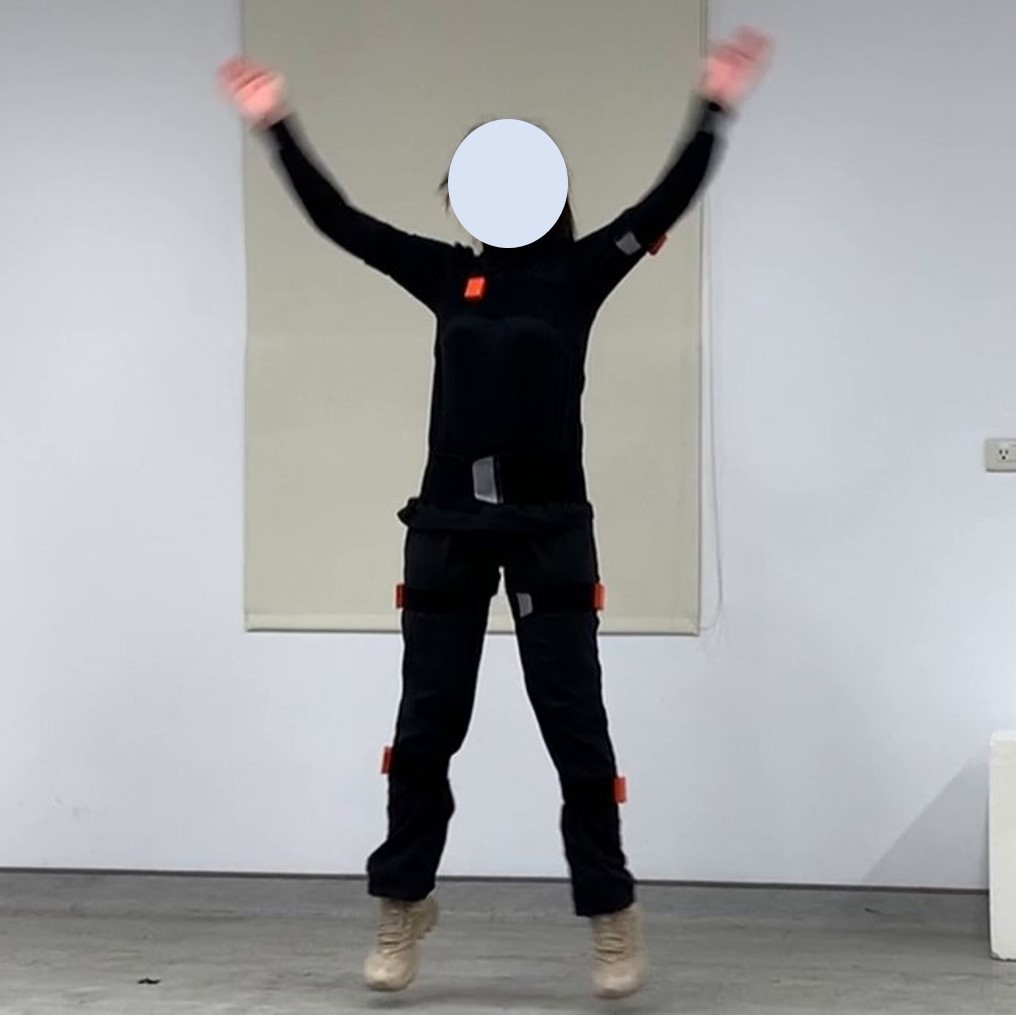
\includegraphics[width=.95\linewidth]{figure/ch4_fig_jump_cam01_with1.jpg}
      \caption*{(a) cam01 真實影像}
    \end{minipage}%
    \begin{minipage}{.5\textwidth}
       \centering
       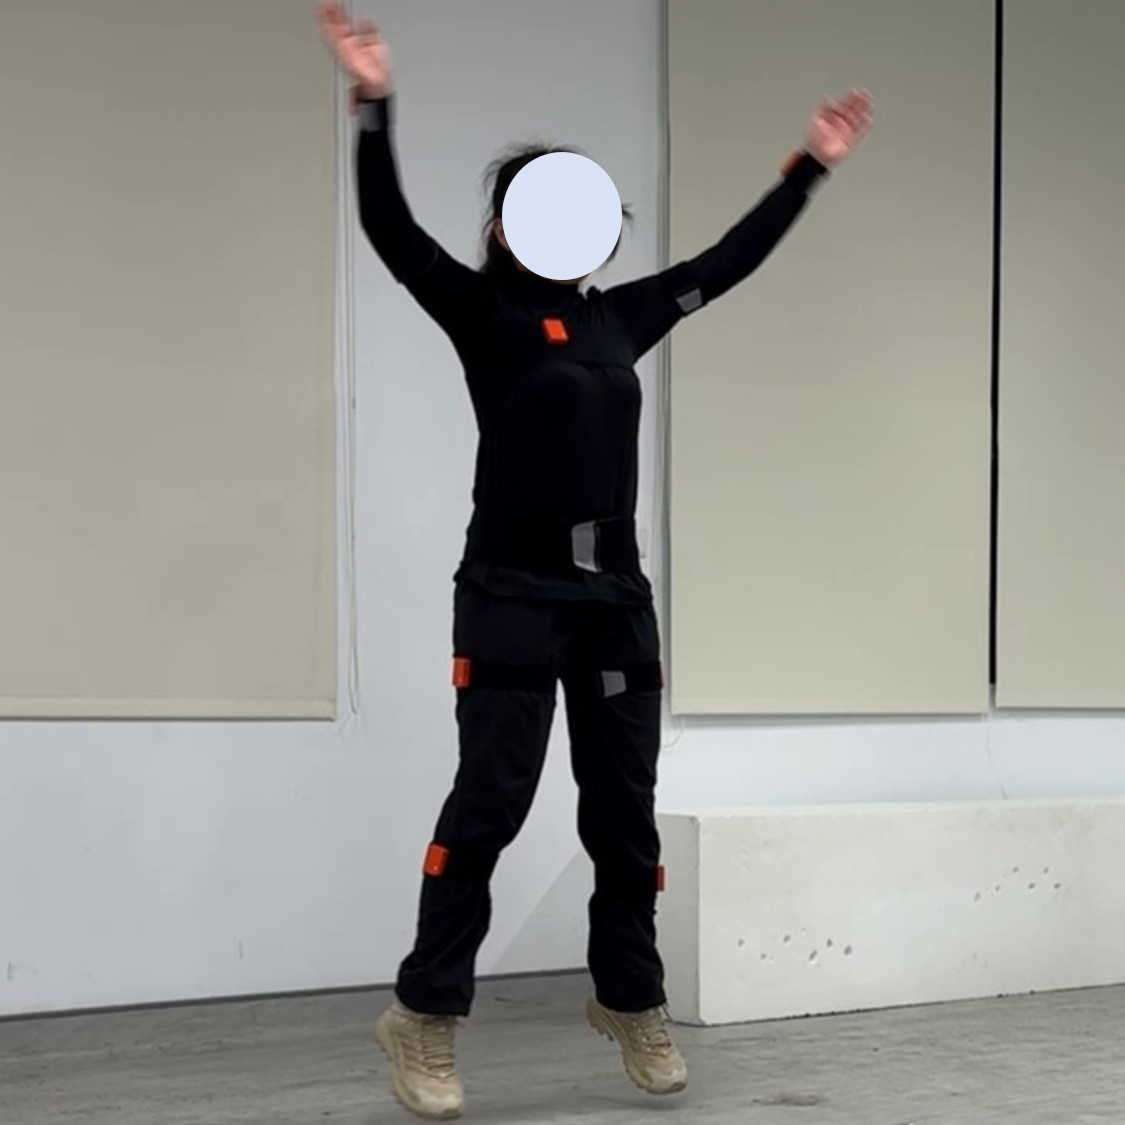
\includegraphics[width=.95\linewidth]{figure/ch4_fig_jump_cam02_with1.jpg}
       \caption*{(b) cam02 真實影像}
    \end{minipage}
    \begin{minipage}{.5\textwidth}
       \centering
       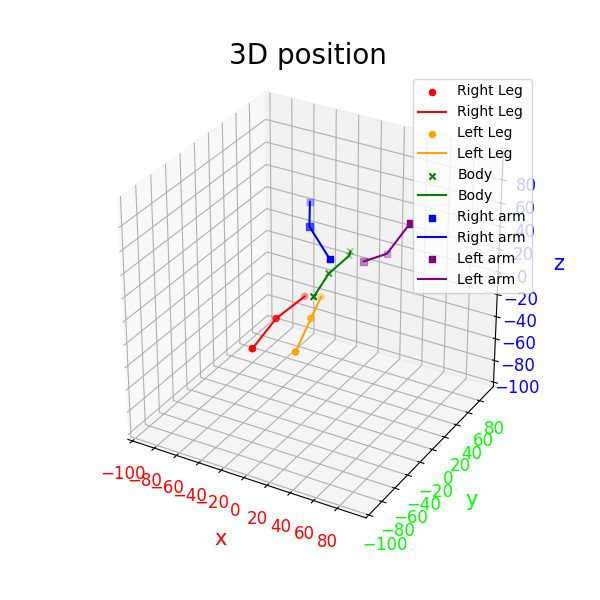
\includegraphics[width=.95\linewidth]{figure/ch4_fig_jump_result_with1.png}
       \caption*{(c) 影像辨識融合 IMU 重建結果}
    \end{minipage}%
    \begin{minipage}{.5\textwidth}
       \centering
       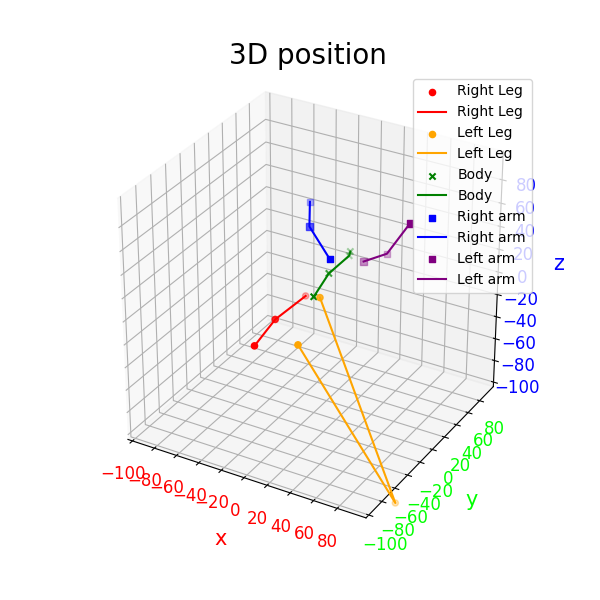
\includegraphics[width=.95\linewidth]{figure/ch4_fig_jump_result_no1.png}
       \caption*{(d) 影像辨識重建結果}
    \end{minipage}
   \caption[開合跳中跳起時的重建結果]{開合跳中跳起時的重建結果}
   \label{ch4_fig_jump_jump}
\end{figure}

\clearpage

落地時的實驗結果如圖~\ref{ch4_fig_jump_stand} 所示,(a)、(b) 為同一時刻點的 cam01 影像及 cam02 影像,(c) 為使用影像辨識融合 IMU 資訊的人體重建結果,(d) 為僅使用影像辨識的人體重建結果。

\begin{figure}[!ht]
   \centering
   \begin{minipage}{.5\textwidth}
      \centering
      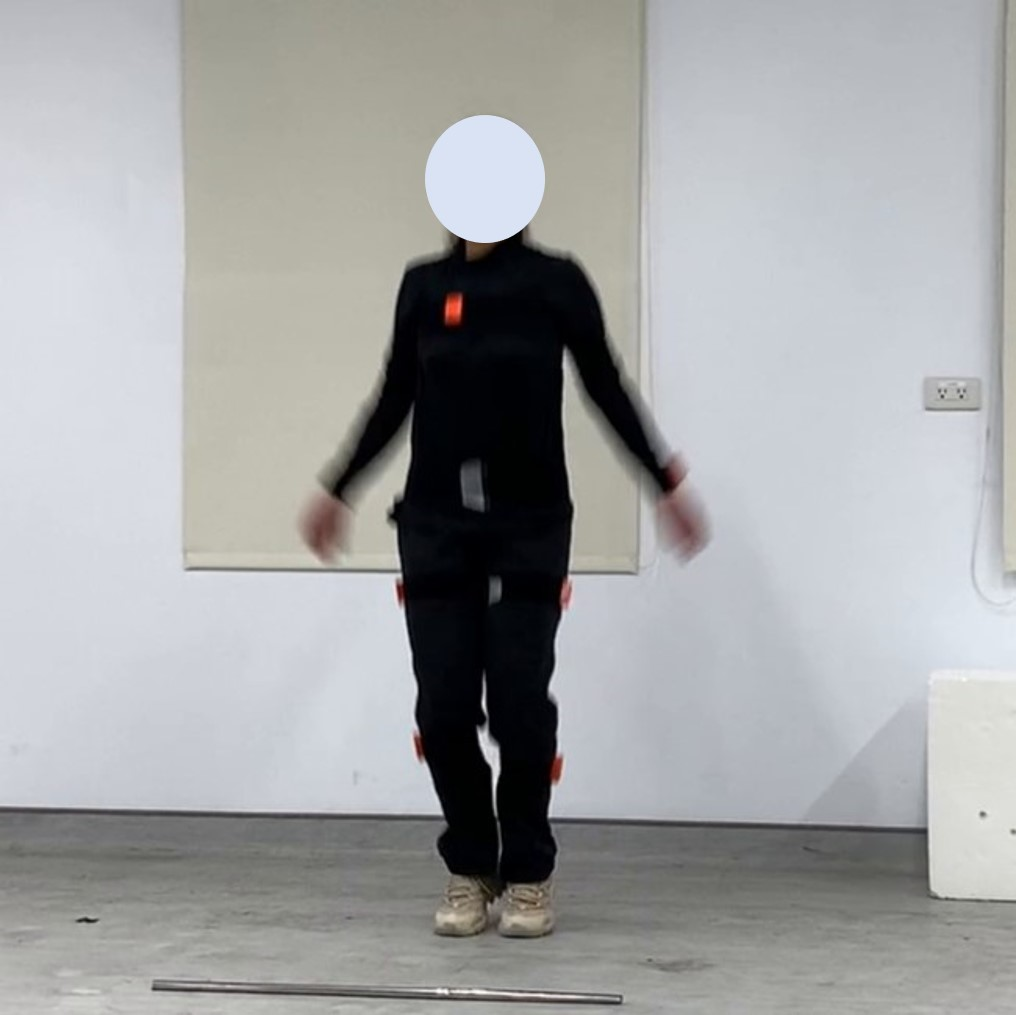
\includegraphics[width=.95\linewidth]{figure/ch4_fig_jump_cam01_with2.jpg}
      \caption*{(a) cam01 真實影像}
    \end{minipage}%
    \begin{minipage}{.5\textwidth}
       \centering
       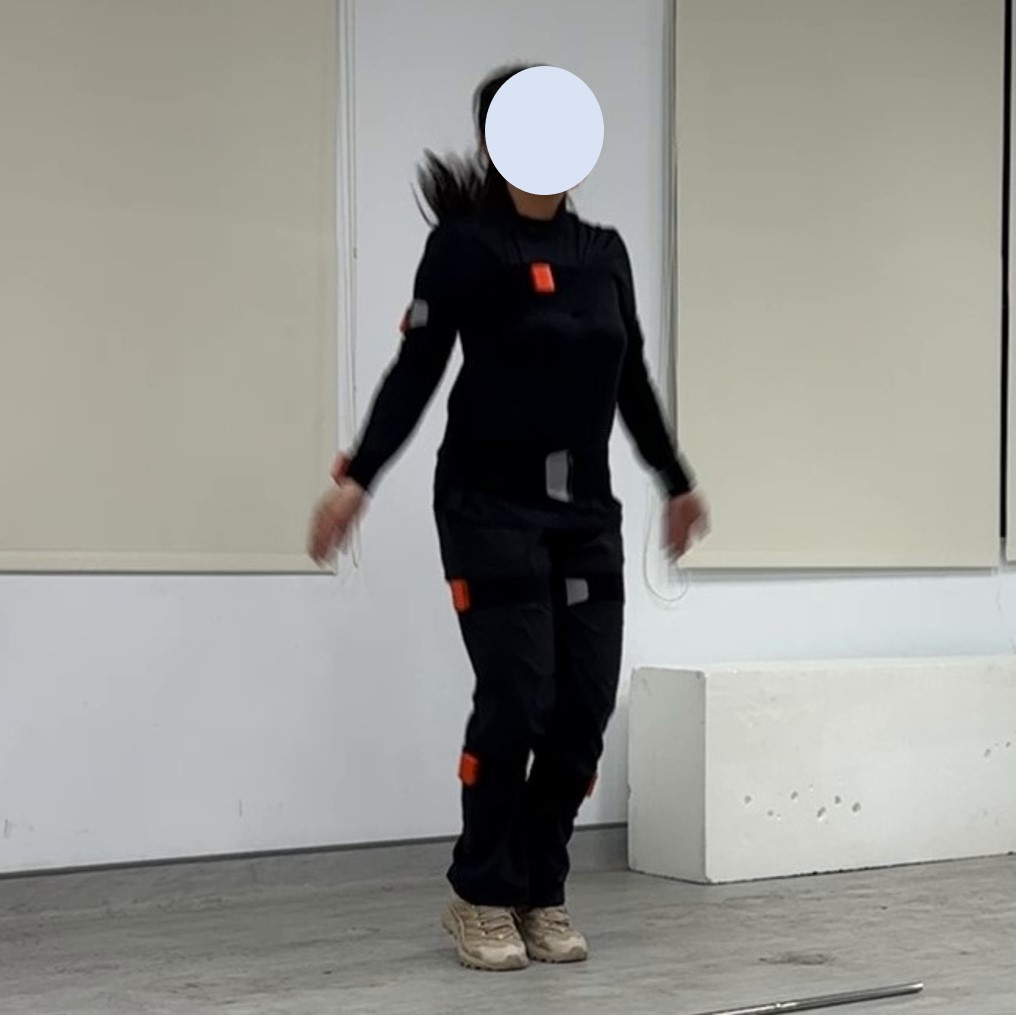
\includegraphics[width=.95\linewidth]{figure/ch4_fig_jump_cam02_with2.jpg}
       \caption*{(b) cam02 真實影像}
    \end{minipage}
    \begin{minipage}{.5\textwidth}
       \centering
       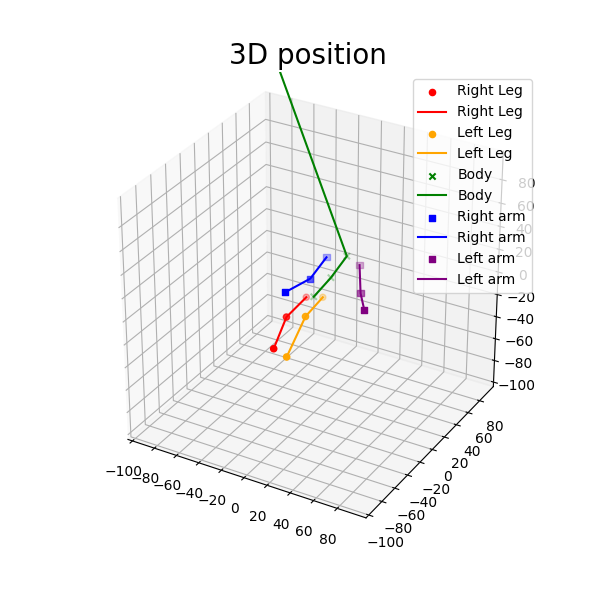
\includegraphics[width=.95\linewidth]{figure/ch4_fig_jump_result_with2.png}
       \caption*{(c) 影像辨識融合 IMU 重建結果}
    \end{minipage}%
    \begin{minipage}{.5\textwidth}
       \centering
       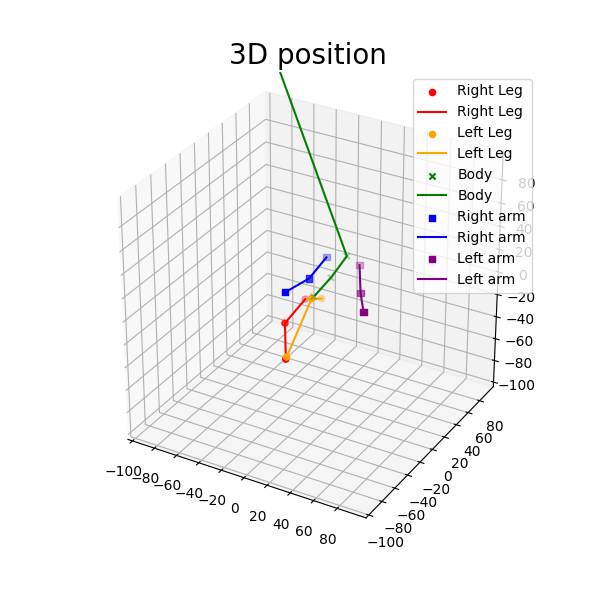
\includegraphics[width=.95\linewidth]{figure/ch4_fig_jump_result_no2.png}
       \caption*{(d) 影像辨識重建結果}
    \end{minipage}
   \caption[開合跳中落地時的重建結果]{開合跳中落地時的重建結果}
   \label{ch4_fig_jump_stand}
\end{figure}

\subsubsection*{開合跳誤差評估}
開合跳實驗總計有 664 幀,每一幀皆估計出人體姿態,每 20 幀進行一次採樣,共計 34 個樣本點進行評估及驗證,可以發現,開合跳實驗中,影像辨識融合 IMU 資訊的肢段的平均估計成功率約 50\%,平均有效誤差約在 80.8609 (mm),僅使用影像辨識的肢段的平均估計成功率約 35.29\%,平均有效誤差約在 76.4560 (mm)。從圖~\ref{ch4_fig_jump_jump}、圖~\ref{ch4_fig_jump_stand} (c)、(d) 可以發現,僅使用影像辨識建立的關節點容易亂飄,影像辨識融合 IMU 朝向資訊的人體重建結果,由於加上朝向的限制,所以較為接近真實人體姿態。
% 而在圖~\ref{ch4_fig_jump_stand} (c)、(d) 中,頭部可以發現頭部的位置點明顯超出邊界。

\clearpage

\subsubsection*{折返跑實驗結果}
% pose_123、314、1045,在300、422可以看到影像辨識把左右邊搞混的現象
折返跑實驗重建中,跑步時的實驗結果如圖~\ref{ch4_fig_run_run} 所示,(a)、(b) 為同一時刻點的 cam01 影像及 cam02 影像,(c) 為使用影像辨識融合 IMU 資訊的人體重建結果,(d) 為僅使用影像辨識的人體重建結果。

\begin{figure}[!ht]
   \centering
   \begin{minipage}{.5\textwidth}
      \centering
      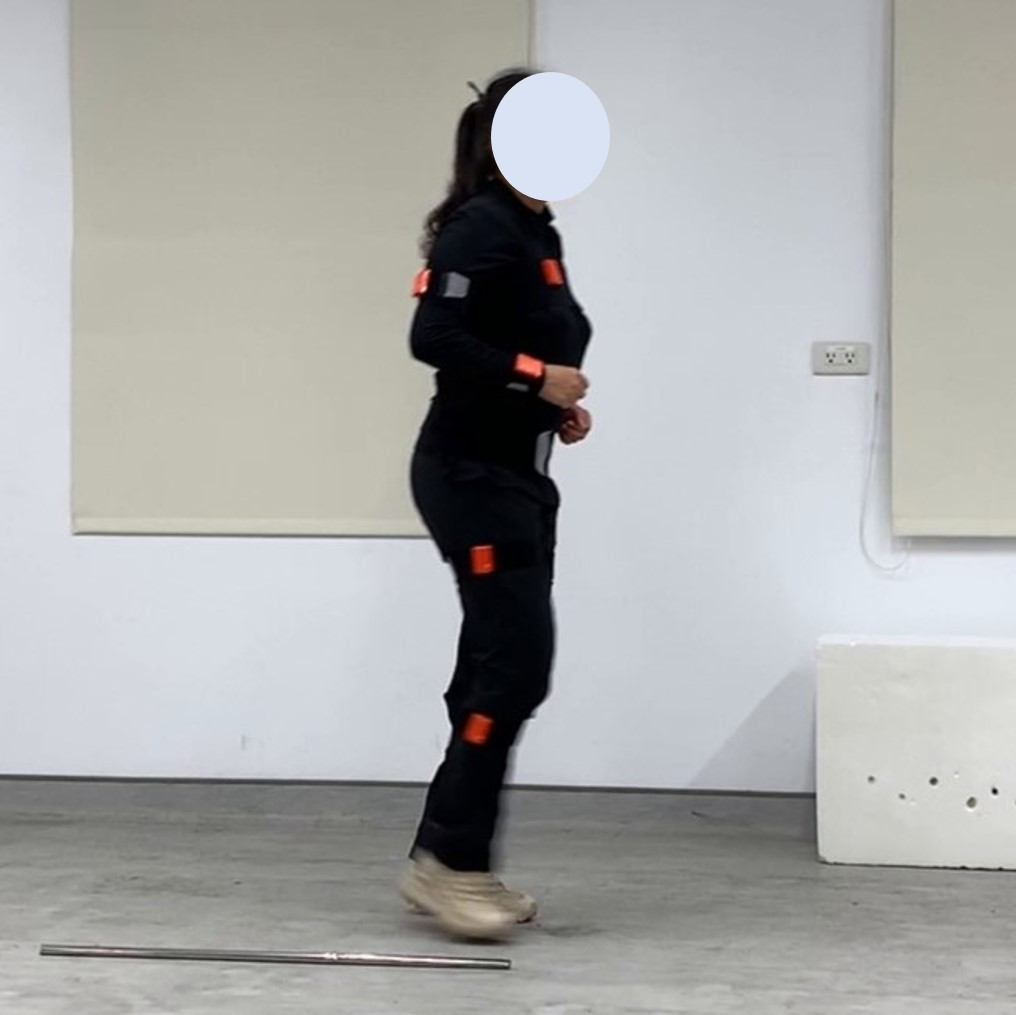
\includegraphics[width=.95\linewidth]{figure/ch4_fig_run_cam01_with1.jpg}
      \caption*{(a) cam01 真實影像}
    \end{minipage}%
    \begin{minipage}{.5\textwidth}
       \centering
       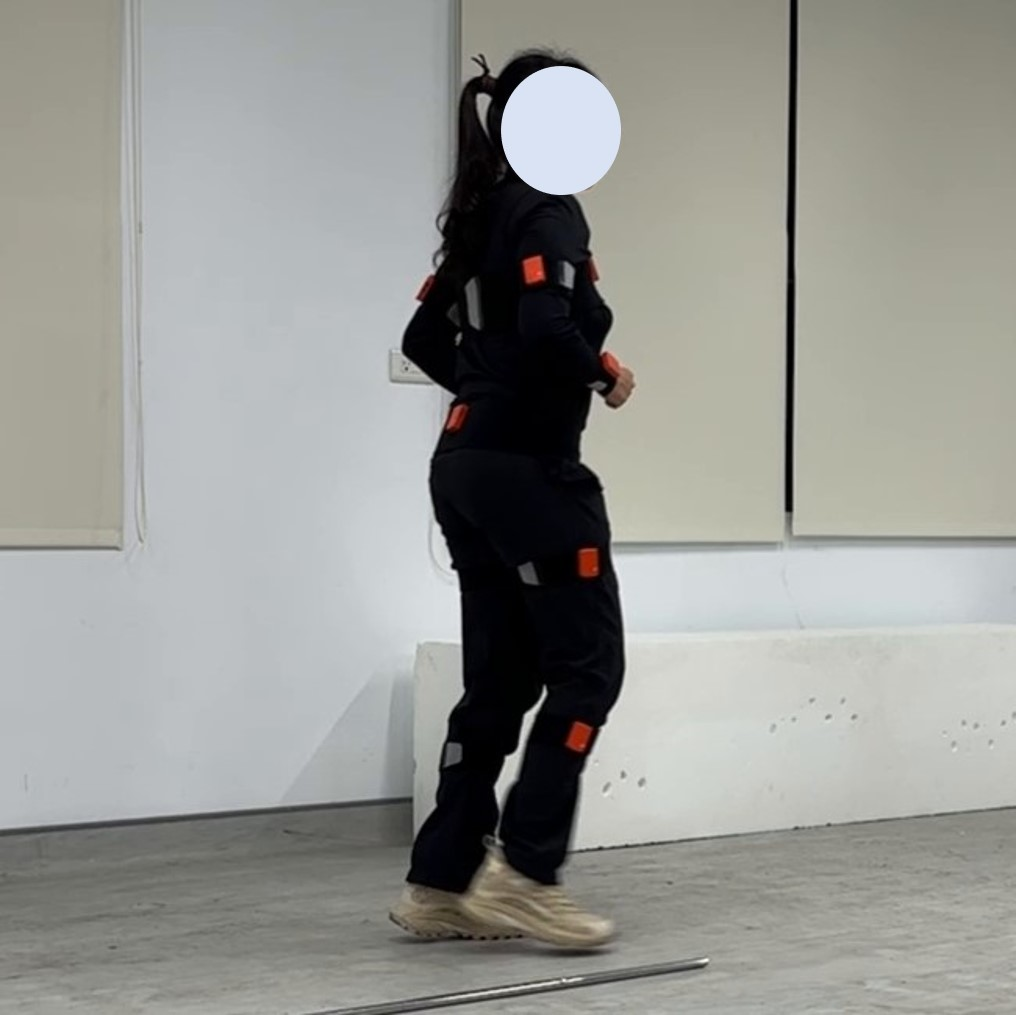
\includegraphics[width=.95\linewidth]{figure/ch4_fig_run_cam02_with1.jpg}
       \caption*{(b) cam02 真實影像}
    \end{minipage}
    \begin{minipage}{.5\textwidth}
       \centering
       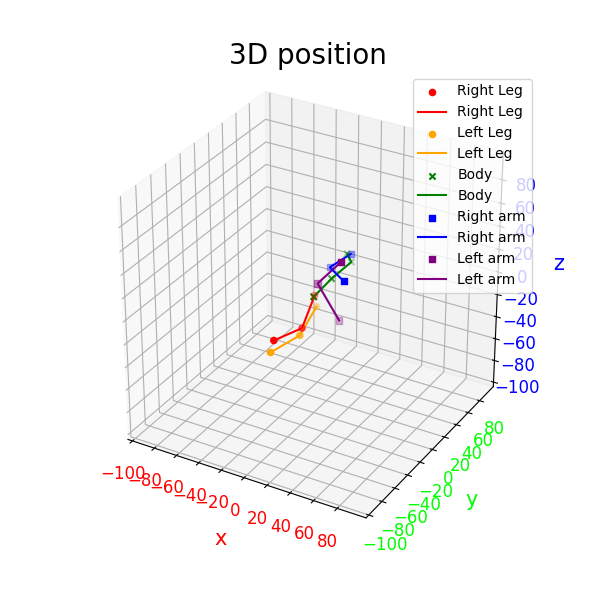
\includegraphics[width=.95\linewidth]{figure/ch4_fig_run_result_with1.png}
       \caption*{(c) 影像辨識融合 IMU 重建結果}
    \end{minipage}%
    \begin{minipage}{.5\textwidth}
       \centering
       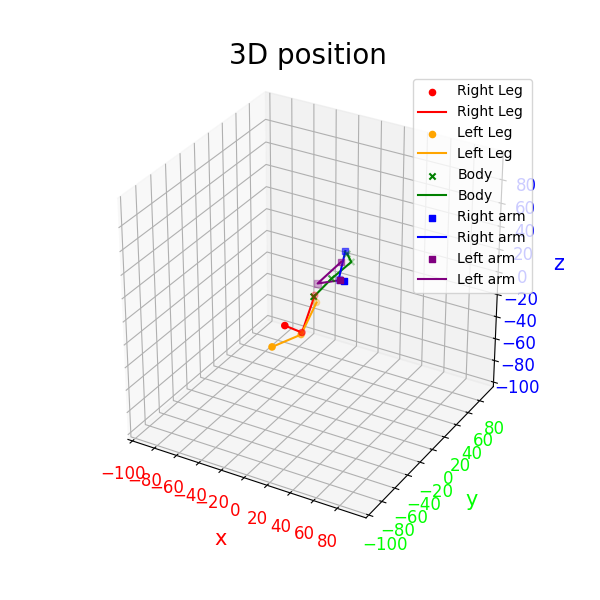
\includegraphics[width=.95\linewidth]{figure/ch4_fig_run_result_no1.png}
       \caption*{(d) 影像辨識重建結果}
    \end{minipage}
   \caption[折返跑中跑步時的重建結果]{折返跑中跑步時的重建結果}
   \label{ch4_fig_run_run}
\end{figure}

\clearpage

轉身時的實驗結果如圖~\ref{ch4_fig_run_turn} 所示,(a)、(b) 為同一時刻點的 cam01 影像及 cam02 影像,(c) 為使用影像辨識融合 IMU 資訊的人體重建結果,(d) 為僅使用影像辨識的人體重建結果。

\begin{figure}[!ht]
   \centering
   \begin{minipage}{.5\textwidth}
      \centering
      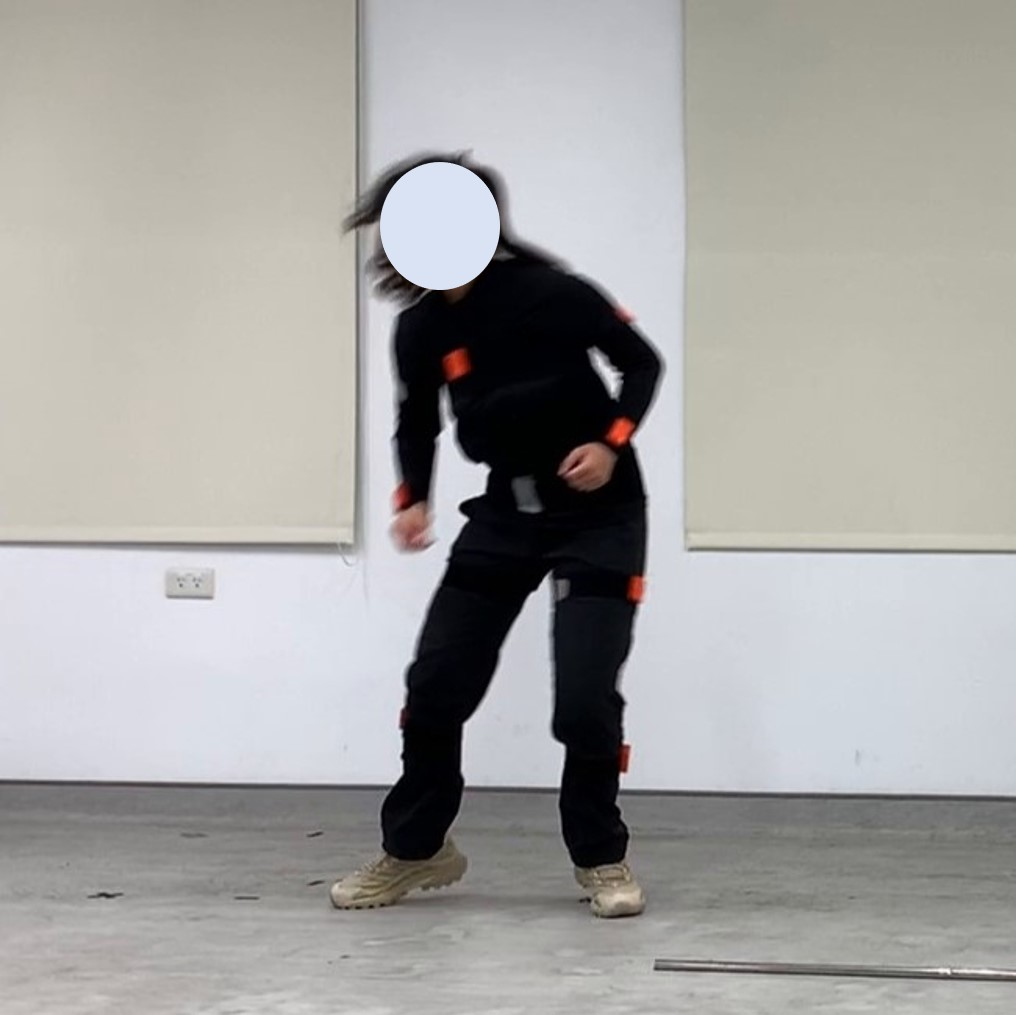
\includegraphics[width=.95\linewidth]{figure/ch4_fig_run_cam01_with2.jpg}
      \caption*{(a) cam01 真實影像}
    \end{minipage}%
    \begin{minipage}{.5\textwidth}
       \centering
       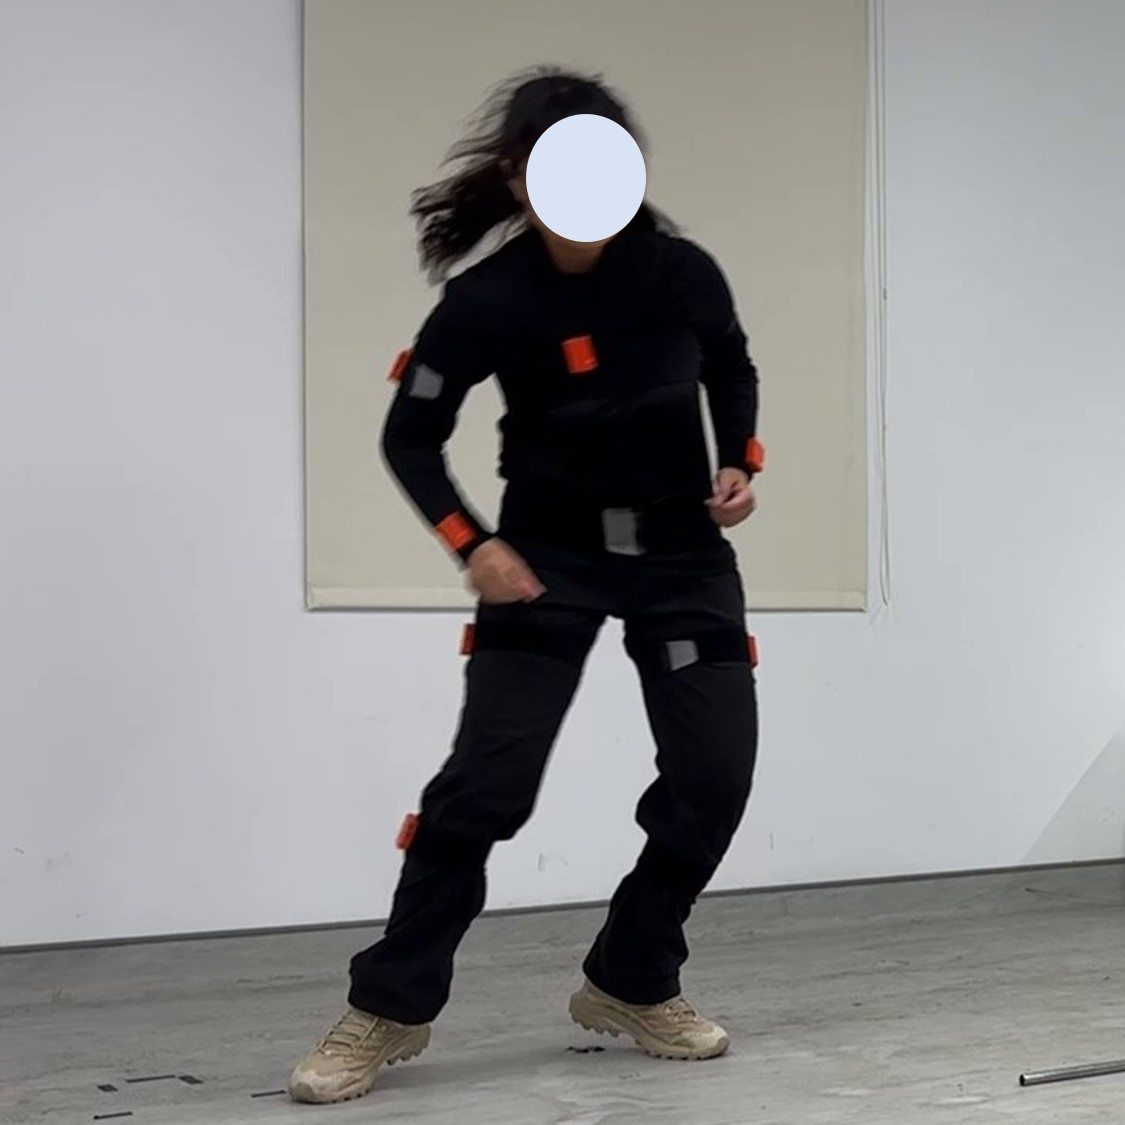
\includegraphics[width=.95\linewidth]{figure/ch4_fig_run_cam02_with2.jpg}
       \caption*{(b) cam02 真實影像}
    \end{minipage}
    \begin{minipage}{.5\textwidth}
       \centering
       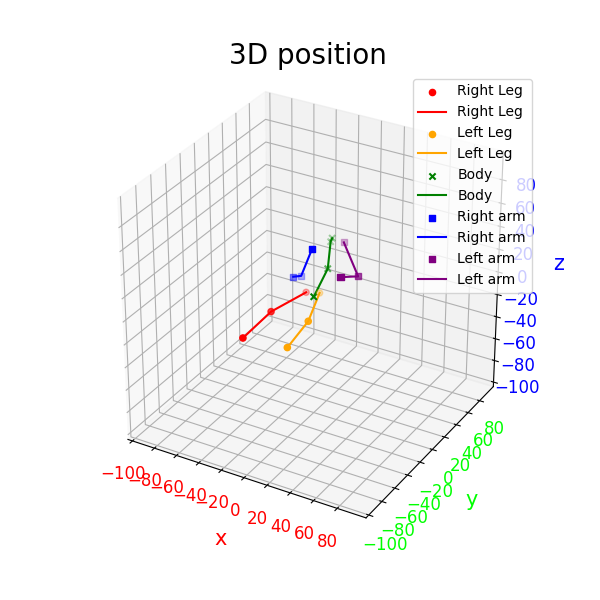
\includegraphics[width=.95\linewidth]{figure/ch4_fig_run_result_with2.png}
       \caption*{(c) 影像辨識融合 IMU 重建結果}
    \end{minipage}%
    \begin{minipage}{.5\textwidth}
       \centering
       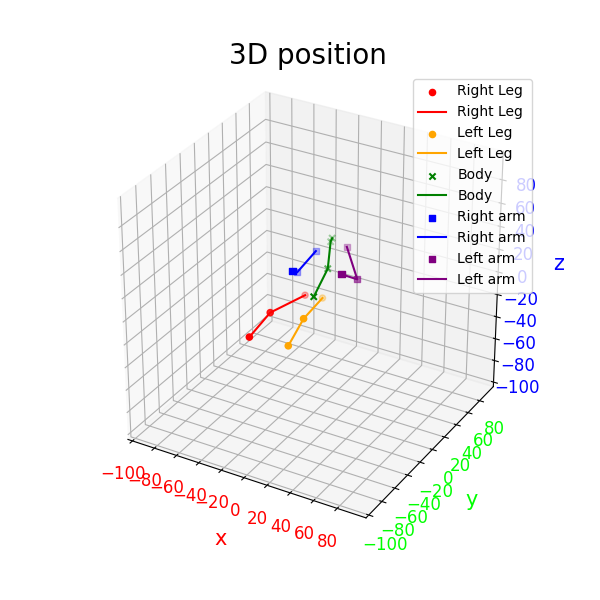
\includegraphics[width=.95\linewidth]{figure/ch4_fig_run_result_no2.png}
       \caption*{(d) 影像辨識重建結果}
    \end{minipage}
   \caption[折返跑中轉身時的重建結果]{折返跑中轉身時的重建結果}
   \label{ch4_fig_run_turn}
\end{figure}

\clearpage

手摸地時的實驗結果如圖~\ref{ch4_fig_run_touch} 所示,(a)、(b) 為同一時刻點的 cam01 影像及 cam02 影像,(c) 為使用影像辨識融合 IMU 資訊的人體重建結果,(d) 為僅使用影像辨識的人體重建結果。

\begin{figure}[!ht]
   \centering
   \begin{minipage}{.5\textwidth}
      \centering
      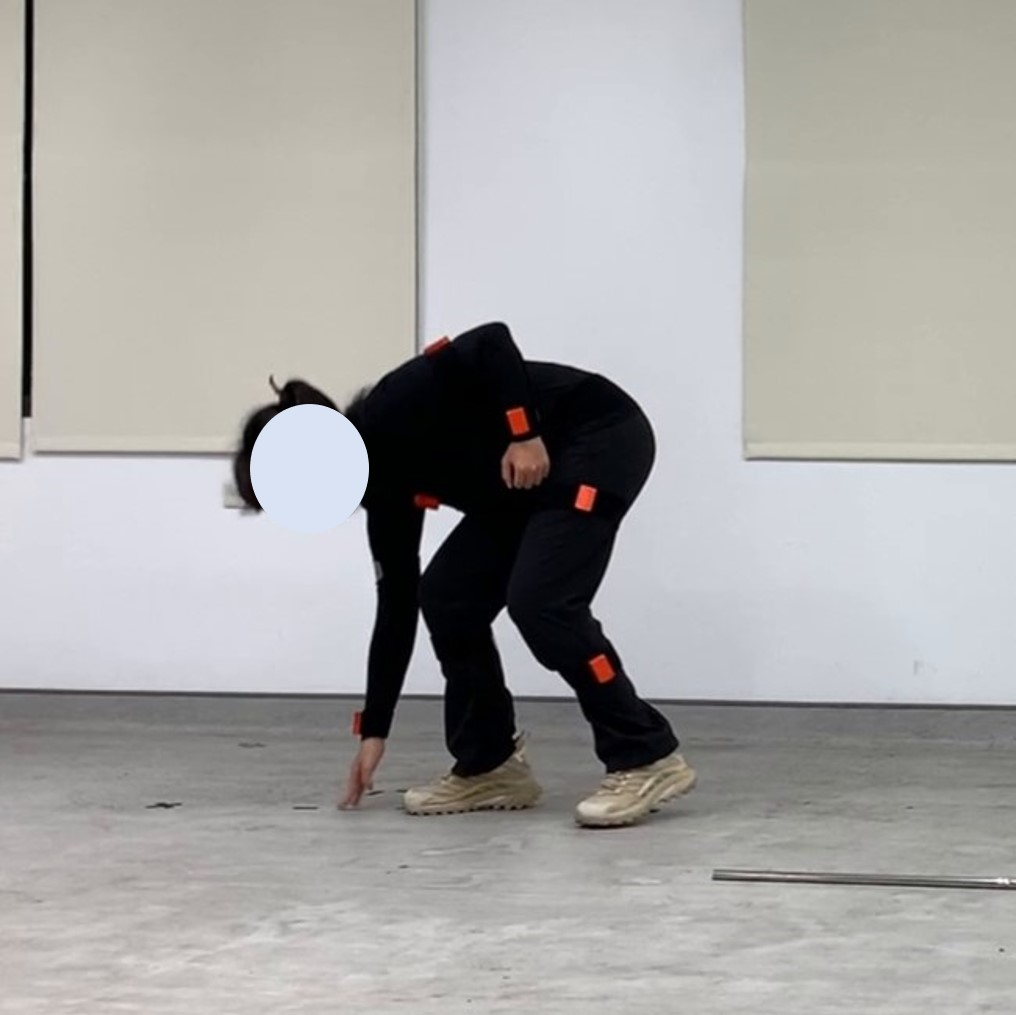
\includegraphics[width=.95\linewidth]{figure/ch4_fig_run_cam01_with3.jpg}
      \caption*{(a) cam01 真實影像}
    \end{minipage}%
    \begin{minipage}{.5\textwidth}
       \centering
       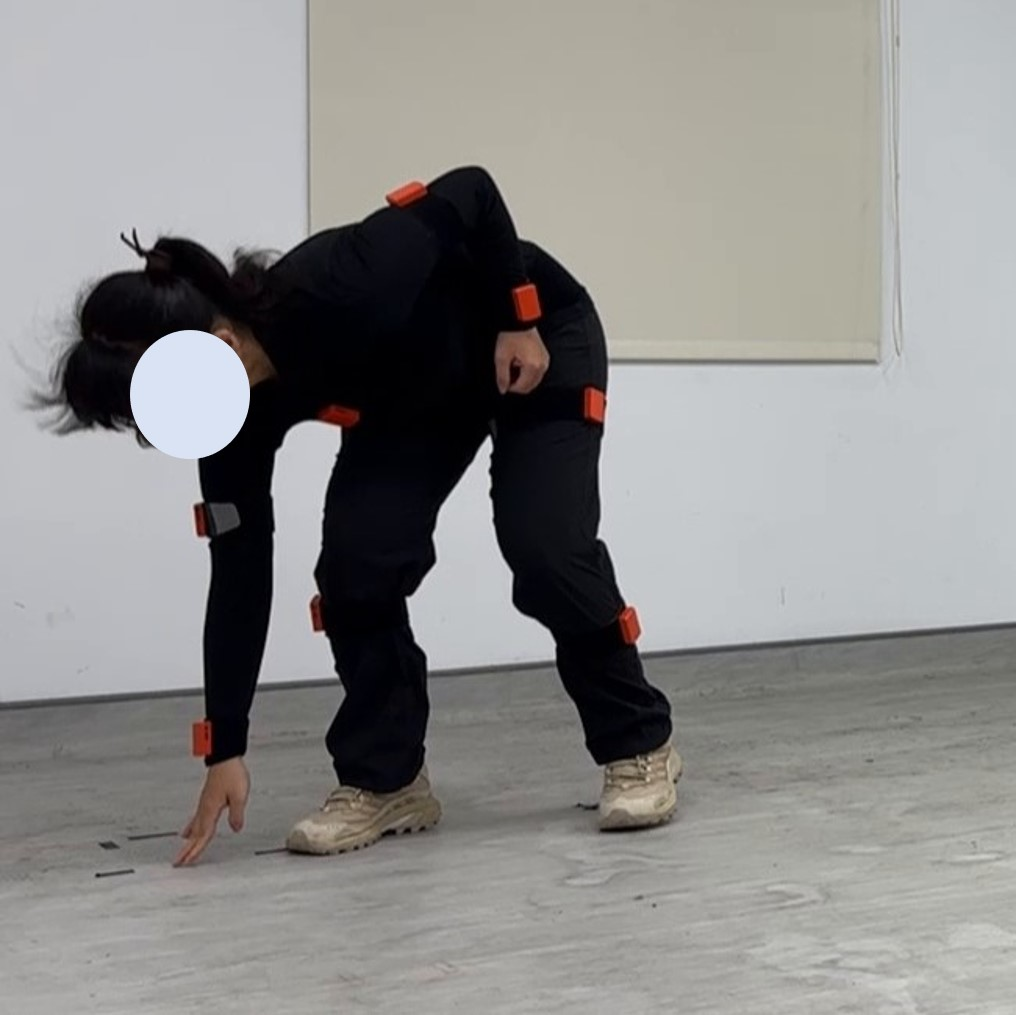
\includegraphics[width=.95\linewidth]{figure/ch4_fig_run_cam02_with3.jpg}
       \caption*{(b) cam02 真實影像}
    \end{minipage}
    \begin{minipage}{.5\textwidth}
       \centering
       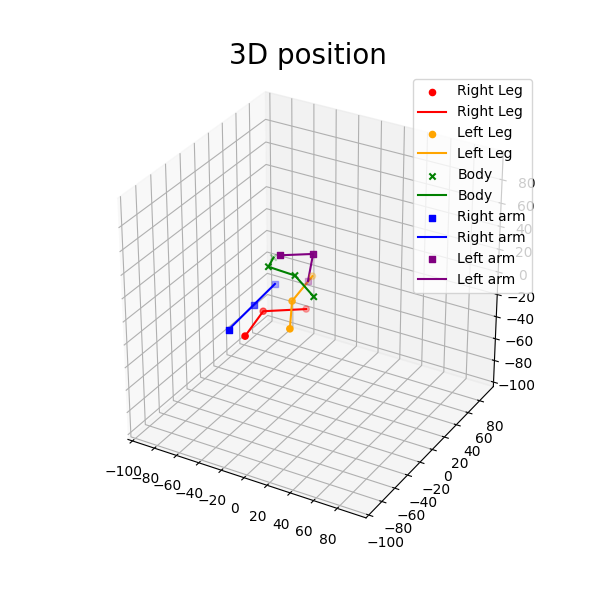
\includegraphics[width=.95\linewidth]{figure/ch4_fig_run_result_with3.png}
       \caption*{(c) 影像辨識融合 IMU 重建結果}
    \end{minipage}%
    \begin{minipage}{.5\textwidth}
       \centering
       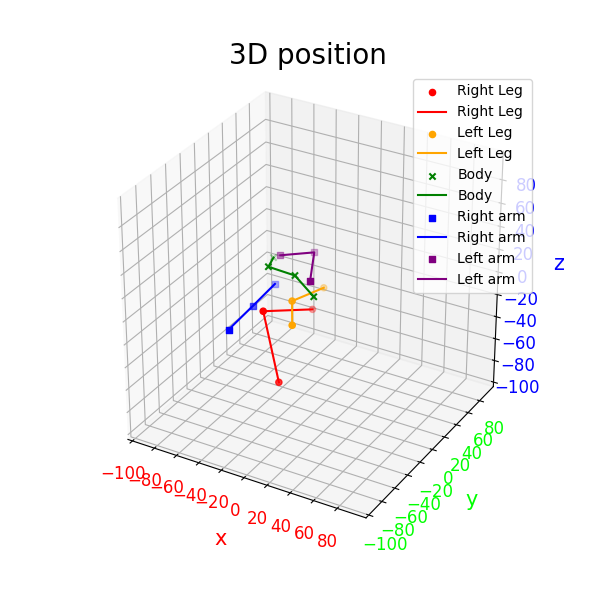
\includegraphics[width=.95\linewidth]{figure/ch4_fig_run_result_no3.png}
       \caption*{(d) 影像辨識重建結果}
    \end{minipage}
   \caption[折返跑中手摸地時的重建結果]{折返跑中手摸地時的重建結果}
   \label{ch4_fig_run_touch}
\end{figure}

\subsubsection*{折返跑誤差評估}
折返跑實驗總計有 1609 幀,每一幀皆估計出人體姿態,每 20 幀進行一次採樣,共計 81 個樣本點進行評估及驗證,可以發現,折返跑實驗中,影像辨識融合 IMU 資訊的肢段的平均估計成功率約 53.09\%,平均有效誤差約在 82.6446 (mm),僅使用影像辨識的肢段的平均估計成功率約 40.74\%,平均有效誤差約在 80.0463 (mm)。從圖~\ref{ch4_fig_run_run}、圖~\ref{ch4_fig_run_turn}、圖~\ref{ch4_fig_run_touch} (c)、(d) 可以發現,影像辨識融合 IMU 朝向資訊的人體重建結果,由於加上朝向的限制,所以較為接近真實人體姿態,且即使是圖~\ref{ch4_fig_run_run} 中,有一半關節被遮擋的情境下也可以成功建立。

\clearpage

\subsubsection*{熱身運動實驗結果}
% pose_594、818、1622、1786,上半身伸展備用410、510、596,肩膀伸展比較屬於正面運動119、151、229、287,腿部拉筋備用778、889,蹲下姿勢1277、1280
熱身運動實驗重建中,腰部伸展時的實驗結果如圖~\ref{ch4_fig_warm_warm} 所示,(a)、(b) 為同一時刻點的 cam01 影像及 cam02 影像,(c) 為使用影像辨識融合 IMU 資訊的人體重建結果,(d) 為僅使用影像辨識的人體重建結果。

\begin{figure}[!ht]
   \centering
   \begin{minipage}{.5\textwidth}
      \centering
      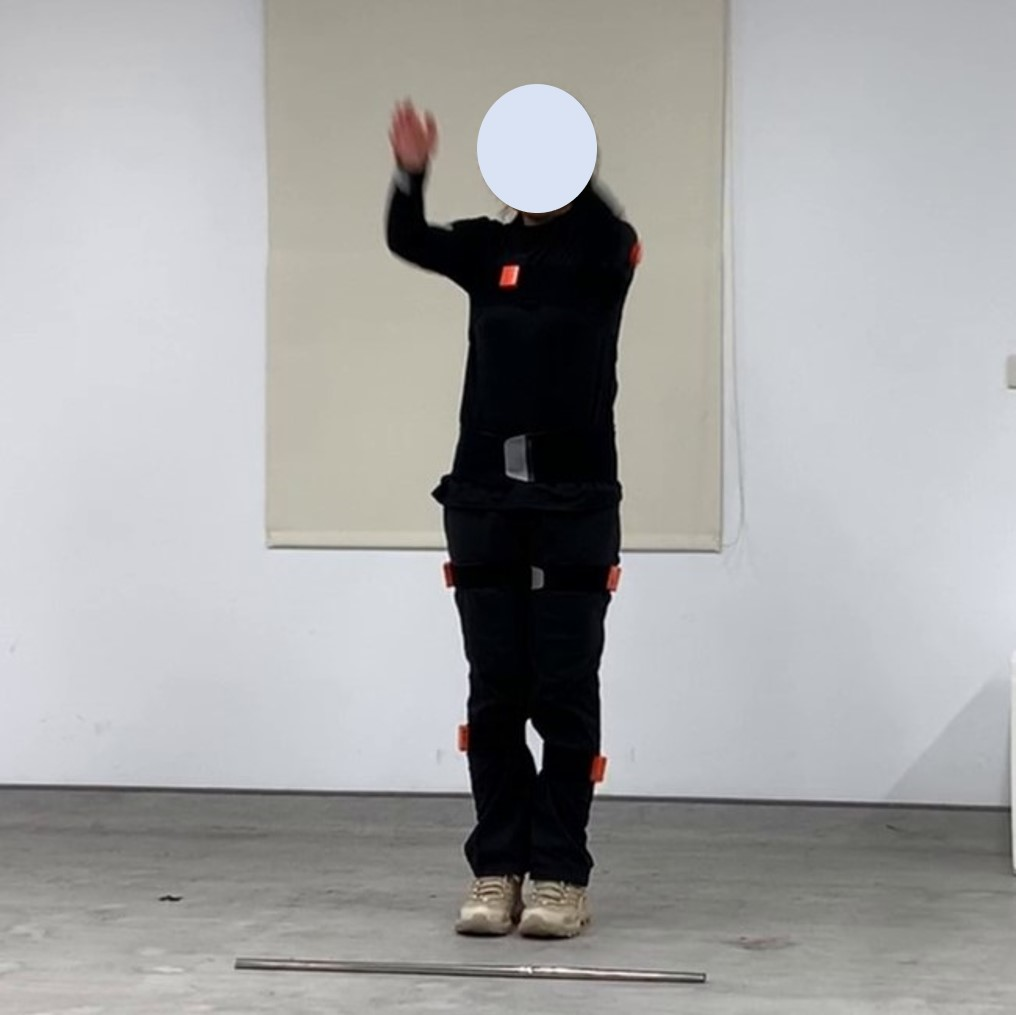
\includegraphics[width=.95\linewidth]{figure/ch4_fig_warm_cam01_with1.jpg}
      \caption*{(a) cam01 真實影像}
    \end{minipage}%
    \begin{minipage}{.5\textwidth}
       \centering
       \includegraphics[width=.95\linewidth]{figure/ch4_fig_warm_cam02_with1.jpg}
       \caption*{(b) cam02 真實影像}
    \end{minipage}
    \begin{minipage}{.5\textwidth}
       \centering
       \includegraphics[width=.95\linewidth]{figure/ch4_fig_warm_result_with1.png}
       \caption*{(c) 影像辨識融合 IMU 重建結果}
    \end{minipage}%
    \begin{minipage}{.5\textwidth}
       \centering
       \includegraphics[width=.95\linewidth]{figure/ch4_fig_warm_result_no1.png}
       \caption*{(d) 影像辨識重建結果}
    \end{minipage}
   \caption[熱身運動中腰部伸展時的重建結果]{熱身運動中腰部伸展時的重建結果}
   \label{ch4_fig_warm_warm}
\end{figure}

\clearpage

腿部伸展側身時的實驗結果如圖~\ref{ch4_fig_warm_side} 所示,(a)、(b) 為同一時刻點的 cam01 影像及 cam02 影像,(c) 為使用影像辨識融合 IMU 資訊的人體重建結果,(d) 為僅使用影像辨識的人體重建結果。

\begin{figure}[!ht]
   \centering
   \begin{minipage}{.5\textwidth}
      \centering
      \includegraphics[width=.95\linewidth]{figure/ch4_fig_warm_cam01_with2.jpg}
      \caption*{(a) cam01 真實影像}
    \end{minipage}%
    \begin{minipage}{.5\textwidth}
       \centering
       \includegraphics[width=.95\linewidth]{figure/ch4_fig_warm_cam02_with2.jpg}
       \caption*{(b) cam02 真實影像}
    \end{minipage}
    \begin{minipage}{.5\textwidth}
       \centering
       \includegraphics[width=.95\linewidth]{figure/ch4_fig_warm_result_with2.png}
       \caption*{(c) 影像辨識融合 IMU 重建結果}
    \end{minipage}%
    \begin{minipage}{.5\textwidth}
       \centering
       \includegraphics[width=.95\linewidth]{figure/ch4_fig_warm_result_no2.png}
       \caption*{(d) 影像辨識重建結果}
    \end{minipage}
   \caption[熱身運動中腿部伸展側身時的重建結果]{熱身運動中腿部伸展側身時的重建結果}
   \label{ch4_fig_warm_side}
\end{figure}

\clearpage

正面腿部伸展時的實驗結果如圖~\ref{ch4_fig_warm_front} 所示,(a)、(b) 為同一時刻點的 cam01 影像及 cam02 影像,(c) 為使用影像辨識融合 IMU 資訊的人體重建結果,(d) 為僅使用影像辨識的人體重建結果。

\begin{figure}[!ht]
   \centering
   \begin{minipage}{.5\textwidth}
      \centering
      \includegraphics[width=.95\linewidth]{figure/ch4_fig_warm_cam01_with3.jpg}
      \caption*{(a) cam01 真實影像}
    \end{minipage}%
    \begin{minipage}{.5\textwidth}
       \centering
       \includegraphics[width=.95\linewidth]{figure/ch4_fig_warm_cam02_with3.jpg}
       \caption*{(b) cam02 真實影像}
    \end{minipage}
    \begin{minipage}{.5\textwidth}
       \centering
       \includegraphics[width=.95\linewidth]{figure/ch4_fig_warm_result_with3.png}
       \caption*{(c) 影像辨識融合 IMU 重建結果}
    \end{minipage}%
    \begin{minipage}{.5\textwidth}
       \centering
       \includegraphics[width=.95\linewidth]{figure/ch4_fig_warm_result_no3.png}
       \caption*{(d) 影像辨識重建結果}
    \end{minipage}
   \caption[熱身運動中正面腿部伸展時的重建結果]{熱身運動中跑步時的重建結果}
   \label{ch4_fig_warm_front}
\end{figure}

\clearpage

背面腿部伸展時的實驗結果如圖~\ref{ch4_fig_warm_back} 所示,(a)、(b) 為同一時刻點的 cam01 影像及 cam02 影像,(c) 為使用影像辨識融合 IMU 資訊的人體重建結果,(d) 為僅使用影像辨識的人體重建結果。

\begin{figure}[!ht]
   \centering
   \begin{minipage}{.5\textwidth}
      \centering
      \includegraphics[width=.95\linewidth]{figure/ch4_fig_warm_cam01_with4.jpg}
      \caption*{(a) cam01 真實影像}
    \end{minipage}%
    \begin{minipage}{.5\textwidth}
       \centering
       \includegraphics[width=.95\linewidth]{figure/ch4_fig_warm_cam02_with4.jpg}
       \caption*{(b) cam02 真實影像}
    \end{minipage}
    \begin{minipage}{.5\textwidth}
       \centering
       \includegraphics[width=.95\linewidth]{figure/ch4_fig_warm_result_with4.png}
       \caption*{(c) 影像辨識融合 IMU 重建結果}
    \end{minipage}%
    \begin{minipage}{.5\textwidth}
       \centering
       \includegraphics[width=.95\linewidth]{figure/ch4_fig_warm_result_no4.png}
       \caption*{(d) 影像辨識重建結果}
    \end{minipage}
   \caption[熱身運動中背面腿部伸展時的重建結果]{熱身運動中背面腿部伸展時的重建結果}
   \label{ch4_fig_warm_back}
\end{figure}

\subsubsection*{熱身運動誤差評估}
熱身運動實驗總計有 2135 幀,每一幀皆估計出人體姿態,每 20 幀進行一次採樣,共計 107 個樣本點進行評估及驗證,可以發現,熱身運動實驗中,影像辨識融合 IMU 資訊的肢段的平均估計成功率約 46.73\%,平均有效誤差約在 7.5974 (mm),僅使用影像辨識的肢段的平均估計成功率約 31.78\%,平均有效誤差約在 67.2949 (mm)。從圖~\ref{ch4_fig_warm_warm}、圖~\ref{ch4_fig_warm_side}、圖~\ref{ch4_fig_warm_front}、圖~\ref{ch4_fig_warm_back} (c)、(d) 可以發現,影像辨識融合 IMU 朝向資訊的人體重建結果,由於加上朝向的限制,所以較為接近真實人體姿態,且即使是圖~\ref{ch4_fig_warm_side} 中,有一半關節被遮擋的情境下也可以成功建立,但在圖~\ref{ch4_fig_warm_back} 中,可以發現重建的效果較差,可能是因為影像辨識模型並沒有被訓練辨識背面的影像,因此影像辨識較難成功。

% \subsubsection*{組合動作實驗結果}
% \subsubsection*{組合動作誤差評估}
\subsection{結論}
% 結論
將以上實驗的成功率與誤差整理成表格,如表~\ref{ch4_tab_conclusion} 所示。
\begin{table}[ht]
   \caption{影像辨識有無融合 IMU 的結果比較}
   \label{ch4_tab_conclusion}
   \centering
   \begin{tabular}{clccccc}
   \toprule
    & IMU 融合 & T pose & 蹲站 & 開合跳 & 折返跑 & 熱身運動 \\
   \midrule
   \multirow{2}{*}{誤差 (mm)} & O & 82.7502 & 76.8410 & 80.8609 & 82.6446 & 75.9740 \\
   & X & 95.0632 & 94.5808 & 76.4561 & 80.0463 & 67.2949 \\
   \midrule
   \multirow{2}{*}{成功率 (\%)} & O & 62.50 & 38.10 & 50.00 & 53.09 & 46.73 \\
   & X & 12.50 & 11.11 & 35.29 & 40.74 & 31.78 \\
   \bottomrule
   \end{tabular}
\end{table}

可以發現,影像辨識融合 IMU 資訊的肢段的平均估計成功率皆高於僅使用影像辨識的肢段,平均約有 23.8\% 的提升,本研究推斷,在 T pose 有顯著提升的原因為在實驗過程中受試者皆靜止不動,相較其他實驗過程中,受試者有執行指定動作,因此 IMU 朝向資訊除量測誤差外的其餘誤差較小,因此加上 IMU 的朝向資訊後,成功率有顯著提升,如圖~\ref{ch4_fig_error_success} (a) 所示。而影像辨識融合 IMU 資訊的肢段的平均有效誤差在 T pose 實驗與蹲站實驗的誤差比較中,影像辨識融合 IMU 資訊重建人體姿態相較僅使用影像辨識重建人體姿態有約 10 (mm) 的改善,而在開合跳、折返跑、熱身運動中,影像辨識融合 IMU 資訊重建人體姿態相較僅使用影像辨識重建人體姿態誤差約提升 5 \textasciitilde\ 10 (mm),如圖~\ref{ch4_fig_error_success} (b) 所示。整體而言,將影像辨識結果融合 IMU 後,無論是誤差有所改善或是沒有明顯增加,在重建成功率上都有所提升,因此本研究推斷,影像辨識融合 IMU 資訊的方法可以提升影像辨識的成功率,且改善影像辨識的重建結果。

\begin{figure}[!ht]
   \centering
   \begin{minipage}{\textwidth}
     \centering
     \includegraphics[width=\linewidth]{figure/ch4_fig_error.png}
     \caption*{(a) 誤差}
   \end{minipage}
   \begin{minipage}{\textwidth}
      \centering
      \includegraphics[width=\linewidth]{figure/ch4_fig_success.png}
      \caption*{(b) 重建成功率}
   \end{minipage}
   \caption[是否融合 IMU 的誤差及成功率比較]{是否融合 IMU 的誤差及成功率比較}
   \label{ch4_fig_error_success}
\end{figure}

\clearpage

% % ------------------------- 4.5 ------------------------- %
% \section{使用影像辨識融合 IMU 於室外估計姿態}
% sensor fusion 在室外的結果
% \subsection{實驗設定}
% % 實驗設定
% 123123
% % \subsection{實驗執行}
% % % 實驗執行
% % 123123
% \subsection{誤差評估}
% % 誤差評估
% 123123
% \subsection{結論}
% % 結論
% 123123

% ------------------------- 4.5 ------------------------- %
\section{小結}
% 回顧;下章節再討論;從驗證結果證實方法有效
本章節首先透過先前學者們提出的資料集與影像辨識融合 IMU 方法,探討減少相機使用數量對於人體姿態估計精準度的影響,若容許誤差 100 (mm),則可以選擇兩台相機或三台相機進行姿勢估計。此外,本研究提出使用影像辨識及三角測量計算方法建立三維人體模型,用於將 IMU 朝向資訊轉換為位置資訊,並透過先前學者們提出的資料集進行驗證,整體平均誤差約為 25.75 (mm)。最後本研究透過開合跳、折返跑、熱身運動等實驗,驗證融合 IMU 資訊是否對於影像辨識重建人體姿態有所改善,結果顯示,影像辨識融合 IMU 的方法可以提升影像辨識的成功率,且改善影像辨識的重建結果,因此本研究推斷,影像辨識融合 IMU 資訊的方法可以提升影像辨識的成功率,且改善影像辨識的重建結果。下一章將統整本研究的結論及貢獻,並提出相關的未來工作。

\clearpage